%% LyX 2.3.4.2 created this file.  For more info, see http://www.lyx.org/.
%% Do not edit unless you really know what you are doing.
\documentclass[12pt,english,review,authoryear,times]{elsarticle}
\usepackage{amsmath}
\usepackage{amsbsy}
\usepackage{fontspec}
\usepackage{unicode-math}
\setmainfont[Mapping=tex-text]{Georgia}
\setcounter{secnumdepth}{2}
\setcounter{tocdepth}{4}
\usepackage{booktabs}
\usepackage{setspace}
\usepackage{esint}
\doublespacing

\makeatletter

%%%%%%%%%%%%%%%%%%%%%%%%%%%%%% LyX specific LaTeX commands.
%% Because html converters don't know tabularnewline
\providecommand{\tabularnewline}{\\}

%%%%%%%%%%%%%%%%%%%%%%%%%%%%%% User specified LaTeX commands.
\usepackage{lineno,hyperref}
\modulolinenumbers[5]
\usepackage{xcolor}
\usepackage{soul}
\setmainfont{EB Garamond}
\graphicspath{{figures/pdflatex/}{../figures/pdflatex/}}

\makeatother

\usepackage{polyglossia}
\setdefaultlanguage[variant=american]{english}
\begin{document}

\begin{frontmatter}{}

\title{Numerical investigation of two-phase flow in high-permeability porous
media: Effect of permeability variation on the surface force between
phases}

\author{Maxime Cochennec\fnref{myfootnote,myfootnote1}}

\author{Hossein Davarzani\fnref{myfootnote}}

\author{Yohan Davit\fnref{myfootnote1}}

\author{Ioannis Igniatiadis\fnref{myfootnote}}

\author{Michel Quintard\fnref{myfootnote1}}

\fntext[myfootnote]{French Geological Survey}

\fntext[myfootnote1]{Institut de Mécanique des Fluides de Toulouse}
\begin{abstract}
The macroscopic description of two-phase flow in porous media requires
modeling the force of interaction between the phases, i.e. the two
fluids and the solid phase. The flow regimes specific to high permeability
porous media are characterized by a non-negligible extent of the interface
between the two fluids, compared to the fluid-solid interface. This
argues for the systematic introduction of the fluid-fluid interaction
terms, i.e. surface integrals also called traction, in the macroscopic
momentum equations. However, we do not know whether these terms are
always non-negligible for this type of flow regime, for example in
cases where the friction with the solid becomes very large. Here we
assess that the share of the traction between the fluids in the overall
pressure drop increases when the flow is more confined, and thus the
friction with the solid phase increases. The idea of solving modified
2D-Stokes equations with a supplementary Darcy term allowed us to
modify the absolute permeability of the structure without having to
modify the geometry per se. Our results demonstrate that the absolute
permeability of the structure does not prejudge the importance of
the traction between fluids in the total pressure drop as long as
the flow regime is characteristic of flow in high permeability porous
media.
\end{abstract}

\end{frontmatter}{}

\linenumbers


\section{Introduction}

\subsection{Two-phase flow in high-permeability porous media}

An accurate description of two-phase flow in high-permeability porous
media is of major importance for several practical applications. One
can mention, among others, soil remediation in gravely soils \citep{fetter2017contaminant},
nuclear safety \citep{clavier2017modeling} or hydrodynamic of catalytic
fixed bed reactors \citep{Santos1991}. However, most of the literature
is dedicated to two-phase flow in low-permeability porous media.

Due to the larger pore size, two-phase flow in high-permeability porous
media (hereafter, high-permeability porous media refers to media for
which the characteristic particle diameter is about one millimeter
and above) results in a complex interaction between capillary, gravity
and viscous forces \citep{davit2018one}. For low-permeability porous
media, the flow is usually dominated by surface tension force, i.e.
the capillary number is low, usually inferior to $10^{-3}$, and the
fluid repartition pattern is well described as two independent flow
streams separate by a multitude of stable meniscus at steady state,
as illustrated in Fig.~\ref{fig:fluidPatterns} (a) \citep{dullien2012porous}.
This regime is characterized by the small extent of the fluid-fluid
interface, as the fluid phases are segregated, with the wetting phase
flowing into the larger pores while the wetting phase occupies the
smaller pores. In contrast, for high permeability porous media, the
flow is no longer capillary-dominated and the viscous forces become
significant (also gravity and inertial effects may become important
if Bond and Reynolds numbers are high, respectively). Thus the fluids
repartition patterns can take two forms, either the non-wetting phase
is continuous, see as an example Fig.~\ref{fig:fluidPatterns} (b),
or is flowing as droplets or ganglia, as in Fig.~\ref{fig:fluidPatterns}
(c). For these two options, the wetting phase is flowing as a film
in contact with the solid and the non-wetting phase flows at the center
of the pores surrounded by the wetting phase. Strictly speaking, these
different regimes must be considered when attempting to describe two-phase
flows with continuous macroscopic equations. Indeed, it has been shown
several times that the overall flow properties depend on the flow
regimes \citep{Avraam1995a,armstrong2016beyond}. At first glance,
one would consider that the exchange terms between the fluids, through
their common surfaces, as negligible compared to their counterpart
between the fluid phases and the solid phase for surface-tension dominated
flow since the extent of the fluid-fluid interface is small. On the
other hand, and this is what we are interested in here, this is not
necessarily the case for regimes specific to flow in high-permeability
porous media for which the extent of the fluid-fluid interface is
large. This is important because, as discussed in the next section,
these exchange terms between phases are the basis of any attempt to
establish continuous relationships on a macroscopic scale starting
from the pore scale.

\begin{figure}
\begin{centering}
%% Creator: Inkscape inkscape 0.92.4, www.inkscape.org
%% PDF/EPS/PS + LaTeX output extension by Johan Engelen, 2010
%% Accompanies image file 'dessin.pdf' (pdf, eps, ps)
%%
%% To include the image in your LaTeX document, write
%%   \input{<filename>.pdf_tex}
%%  instead of
%%   \includegraphics{<filename>.pdf}
%% To scale the image, write
%%   \def\svgwidth{<desired width>}
%%   \input{<filename>.pdf_tex}
%%  instead of
%%   \includegraphics[width=<desired width>]{<filename>.pdf}
%%
%% Images with a different path to the parent latex file can
%% be accessed with the `import' package (which may need to be
%% installed) using
%%   \usepackage{import}
%% in the preamble, and then including the image with
%%   \import{<path to file>}{<filename>.pdf_tex}
%% Alternatively, one can specify
%%   \graphicspath{{<path to file>/}}
%% 
%% For more information, please see info/svg-inkscape on CTAN:
%%   http://tug.ctan.org/tex-archive/info/svg-inkscape
%%
\begingroup%
  \makeatletter%
  \providecommand\color[2][]{%
    \errmessage{(Inkscape) Color is used for the text in Inkscape, but the package 'color.sty' is not loaded}%
    \renewcommand\color[2][]{}%
  }%
  \providecommand\transparent[1]{%
    \errmessage{(Inkscape) Transparency is used (non-zero) for the text in Inkscape, but the package 'transparent.sty' is not loaded}%
    \renewcommand\transparent[1]{}%
  }%
  \providecommand\rotatebox[2]{#2}%
  \newcommand*\fsize{\dimexpr\f@size pt\relax}%
  \newcommand*\lineheight[1]{\fontsize{\fsize}{#1\fsize}\selectfont}%
  \ifx\svgwidth\undefined%
    \setlength{\unitlength}{373.15993422bp}%
    \ifx\svgscale\undefined%
      \relax%
    \else%
      \setlength{\unitlength}{\unitlength * \real{\svgscale}}%
    \fi%
  \else%
    \setlength{\unitlength}{\svgwidth}%
  \fi%
  \global\let\svgwidth\undefined%
  \global\let\svgscale\undefined%
  \makeatother%
  \begin{picture}(1,0.3143455)%
    \lineheight{1}%
    \setlength\tabcolsep{0pt}%
    \put(0,0){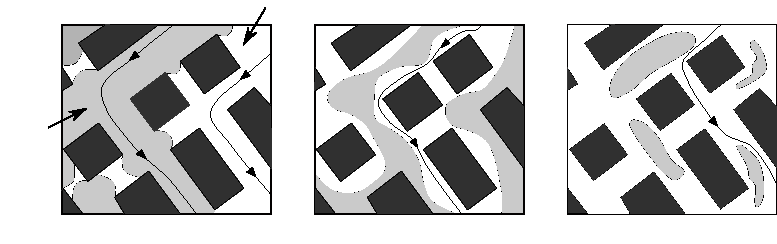
\includegraphics[width=\unitlength,page=1]{dessin.pdf}}%
    \put(0.20241606,0.00226949){\color[rgb]{0,0,0}\makebox(0,0)[lt]{\lineheight{1.25}\smash{\begin{tabular}[t]{l}(a)\end{tabular}}}}%
    \put(0.52734711,0.00226111){\color[rgb]{0,0,0}\makebox(0,0)[lt]{\lineheight{1.25}\smash{\begin{tabular}[t]{l}(b)\end{tabular}}}}%
    \put(0.85316917,0.00226949){\color[rgb]{0,0,0}\makebox(0,0)[lt]{\lineheight{1.25}\smash{\begin{tabular}[t]{l}(c)\end{tabular}}}}%
    \put(0.34787504,0.3013149){\color[rgb]{0,0,0}\makebox(0,0)[lt]{\lineheight{1.25}\smash{\begin{tabular}[t]{l}fluid 2\end{tabular}}}}%
    \put(-0.00039359,0.12182006){\color[rgb]{0,0,0}\makebox(0,0)[lt]{\lineheight{1.25}\smash{\begin{tabular}[t]{l}fluid 1\end{tabular}}}}%
  \end{picture}%
\endgroup%

\par\end{centering}
\caption{Illustration of possible fluids dispatching in a 2D porous network
with solid phase in black, fluid 1, that stands for the non-wetting
phase (gray) and the wetting fluid (white), (a) the two fluids are
flowing in different channels separate by numerous meniscus (b) wetting
and non-wetting fluid are flowing together in most of the pores as
two continuous streams and (c) both fluids are flowing together in
most of the pores and the non-wetting phase is discontinuous - Adapted
from \citep{dullien2012porous}\label{fig:fluidPatterns}}
\end{figure}


\subsection{Continuous model}

Volume averaged microscopic equation of motion for two Newtonian fluids
$i,j=o,w$ reads 

\begin{equation}
\rho_{i}\varepsilon_{i}\left(\frac{\partial\mathbf{U}_{i}}{\partial t}+\mathbf{U}_{i}\cdot\nabla\mathbf{U}_{i}\right)=-\varepsilon_{i}\nabla P_{i}+\varepsilon_{i}\rho_{i}\mathbf{g}+\varepsilon_{i}\nabla\cdot\boldsymbol{\tau}_{i}+(\mathbf{F}_{ij}+\mathbf{F}_{is}),\;i\neq j,\label{eq:averagedMomentum}
\end{equation}

where $\varepsilon_{i}=V_{i}/V$ is the volume fraction of the $i$-fluid
and $V$ is a representative elementary volume, $U_{i}$ is the intrinsic
average velocity of the $i$-fluid, $P_{i}$ is the intrinsic average
pressure of the $i$-fluid and $\boldsymbol{\tau}_{i}$ denotes the
average viscous stress tensor. The last two terms in the left hand
side denote the force of interaction per unite volume exerted by fluid
$i$ upon fluid $j$ and the force of interaction per unit volume
exerted by fluid $i$ upon the solid phase, respectively \citep{Kalaydjian1987}. 

From there, there are two possible ways to adress Eq.~\ref{eq:averagedMomentum}
and the associated equations. In volume averaging litterature, one
seeks to express the terms of interaction between the phases with
averaged quantities and to recast equation Eq.~\ref{eq:averagedMomentum}
in a form similar to Darcy's law (equation for creeping saturated
single-phase flow in porous media). Indeed, by considering creeping
two-phase flow Eq.~\ref{eq:averagedMomentum} can be written as

\begin{equation}
0=-\varepsilon_{i}\nabla P_{i}+\varepsilon_{i}\rho_{i}\mathbf{g}+\frac{1}{V}\int_{A_{is}+A_{ij}}\mathbf{n}_{i}\cdot\left(-\mathbf{I}p_{i}+\mu_{i}\left(\nabla\mathbf{u}_{i}+\left(\nabla\mathbf{u}_{i}\right)^{T}\right)\right)\mathrm{d}A.\label{eq:averagedMomentumIntegral}
\end{equation}

where $p_{i}$ and $u_{i}$ are microscopic pressure and velocity
fields of fluid $i$, respectively. By expressing the surface integrals
in term of averaged quantities one can obtain the following momentum
balance equations,

\begin{equation}
\mathbf{U}_{i}=-\frac{1}{\mu_{i}}\mathbf{K}_{ii}^{*}\cdot(\nabla P_{i}-\rho_{i}\mathbf{g})-\frac{1}{\mu_{j}}\mathbf{K}_{ij}^{*}\cdot(\nabla P_{j}-\rho_{j}\mathbf{g}),\quad i,j=o,w\:\mathrm{and}\:i\neq j,\label{eq:darcyCross}
\end{equation}

in which $\mathbf{K}_{ij}^{*}$ are the coupled relative permeability
tensors that pertain to the interaction between the fluids \citep{Whitaker1986a,Lasseux1996}.

The reader is warned that Eq.~\ref{eq:darcyCross} has, to our knowledge,
never been used in practice to model two-phase subsurface flows. On
the contrary, the ubiquitous continuous model used to describe two-phase
flows in soils is based on a direct extension of the Darcy's equation
and the whole model, also known as Muskat equations \citep{wyckoff1936flow,muskat1938flow},
reads

\begin{subequations}\label{eq:muskatModel}

\begin{equation}
0=\frac{\partial\varepsilon S_{i}}{\partial t}+\nabla\cdot\mathbf{U}_{i},\quad i=o,w,
\end{equation}

\begin{equation}
\mathbf{U}_{i}=-\frac{1}{\mu_{i}}\mathbf{K}_{i}\cdot(\nabla P_{i}-\rho_{i}\mathbf{g}),\quad i=o,w,
\end{equation}

\begin{equation}
1=S_{w}+S_{o}
\end{equation}

\begin{equation}
\mathbf{K}_{w}=\mathbf{K}k_{rw}(S_{w}),\qquad\mathbf{K}_{o}=\mathbf{K}k_{ro}(S_{w}),
\end{equation}

\begin{equation}
P_{c}(S_{w})=P_{o}-P_{w}.
\end{equation}

\end{subequations}

where $\mathbf{K}$ is the absolute permeability tensor. The generalization
toward two-phase flows involves the introduction of the relative permeability
terms $k_{ri}$ which account for the division of the void space between
the fluids \citep{dullien2012porous}, thus the relative permeability
depends (non-linearly) only on the saturation. To close the set of
the macroscopic equations a constitutive relation between the macroscopic
pressure of each fluid has to be furnished. This relation is known
as the capillary pressure relation and, as for the relative permeabilities,
is supposed to depends non-linearly only on the saturation \citep{leverett1941capillary}. 

A significant amount of work attempted to make improvements to the
Muskat equations (e.g. including moving contact line \citep{Kalaydjian1987,Hassanizadeh1993,barenblatt2003mathematical}
or take into account the trapped phases \citep{hilfer1998macroscopic}).
Here we would stress that the concept of relative permeabilities into
the Muskat equations is dedicated to independent flow pathways only
\citep{blunt2017multiphase} and the underlying assumption that the
two streams do not interfere with each other, a situation far from
the regimes previously identified for high permeability porous media.
Thus Eq.~\ref{eq:muskatModel}(b) does not take into account the
interaction between the fluids as opposed to Eq.~\ref{eq:darcyCross}.
If the former is used to the detriment of the latter, it is mainly
because the literature on subsurface flow is focused on oil recovery
applications, for which the permeability is very low and the independent
streams regime is a good approximation. 

Another approach, widely used in the literature on two-phase flow
in Trickle Bed Reactor (TBR), is to implement Eq.~\ref{eq:averagedMomentum}
and provide constitutive relations for the interaction terms between
the phases. These relations are usually obtained through interpretation
of experimental data. Some results, focusing on relation for the interaction
between the fluid phases, are given in the next section as well as
results in literature for coupled permeabilities from the porous medium
approach.

\subsection{Modeling of the interaction between fluids}

Based on the generalized Darcy law with coupled terms Eq.~\ref{eq:darcyCross},
experimental works computed the coupled transport coefficient through
steady-state cocurent flow in sandpack with one fluid, and alternatively
the other, which is submitted to a null pressure gradient. This protocol
was used with oil and water in a cylindric sandpack \citep{zarcone1994determination}
and the authors found a negligible effect of the coupled permeabilities
in the overall flow. With the same protocol, with oil and water in
a 2D-sandpack \citet{Dullien1996} found that the coupled permeabilities
are important since they can contribute at best to 35\% of the effective
permeability. Alternatively, authors imposed \citep{ramakrishnan2015measurement}
a null displacement and measured the induced pressure drop, with air
and water in a Berea sandstone core they found that the coupled transport
coefficients must not be overlooked for intermediate saturations.
Several authors conducted experiments with two different set-ups as
proposed by \citet{Rose1988}, see for example \citet{bentsen1993use}
who made cocurrent and countercurrent experiments with water and oil
in a sandpack and found that coupled permeabilities reach, at least,
15\% of the effective permeability value. However, it was pointed
out that the saturation between the two sets of experiments can be
very different and therefore the computed relative permeabilities
can not be safely compared \citep{langaas2001numerical}. The effect
of the non-wetting phase connectivity on the transport parameters
was extensively studied in \citep{Avraam1995}, the authors performed
steady-state cocurrent two-phase flow in 2D-micro model experiments
and found that the contribution of the coupled permeabilities on the
flow is non-negligible and depend on the flow regimes.

Several numerical studies investigated the share of the coupled permeabilities
in the effective permeability. The seminal work of \citet{Rothman1990}
examined the question by conducting two-phase flow simulations in
simple geometries with the immiscible lattice-gas method. The author
found non-negligible participation of the coupled permeabilities by
applying the volume force alternatively on each fluid. Numerous authors
used the lattice-Boltzmann method, such as \citep{Li2005}, in which
the authors examined the value of the coupled permeabilities as a
function of the saturation in a 3D-sphere pack and they found results
in agreement with Rothman's results. \citet{Yiotis2007} used a lattice
Boltzmann method in 2D and 3D pore networks and found a non-wetting
apparent relative permeability greater than unity when the wetting
fluid is more viscous than the non-wetting fluid. This result is a
manifestation of the lubrification effect, also observed in experiments
\citep{odeh1959effect}, and arising because of strong hydraulic coupling
between the fluids. Recently, \citet{shams2018study} have used a
Volume Of Fluid method to study the transport coefficients of fluid
layers in non-circular capillary tubes. Based on analogy with a model
Couette flow the authors have derived simple relations that can predict
with good accuracy the transport coefficients, including the coupled
ones, of fluid layers. We can also refer to recent work in which a
whole analytical model is given for one-dimensional two-phase flow
in coarse non-consolidated porous media and which correctly predicts
the pressure loss in a debris bed \citep{clavier2017modeling}. 

Several correlations from theorical analysis for the fluid-fluid force
interaction have been derived in hydrodynamic of TBR litterature.
These correlations usually relate the momentum exchange between the
fluids to the flow velocity and the medium properties with Ergun's
like relations. For example, \citet{Attou1999} found that the drag
between the fluids can be expressed as follows

\[
F_{lg}=A_{lg}U_{r}+B_{lg}U_{r}^{2},
\]

where the relative velocity is given by $U_{r}=U_{g}-\frac{S_{g}}{S_{l}}U_{l}$
and$A_{lg}$ and $B_{lg}$ are coefficients that depend on the volume
fraction of the gas phase and the medium properties. The subscripts
$g$ and $l$ denote the gas phase and the liquid phase, respectively.
This type of model with explicit account of interaction between fluids,
see also \citep{Tung1988,iliuta2005modelling}, gives good results
when compared with experimental results \citep{Wang2013}. 

\subsection{Outline of the study}

Up to this point we have seen that the macroscopic momentum equations
need the modeling of the force of interaction terms between phases.
The interaction between fluids is neglected in the traditional model
used for the study of subsurface two-phase flow, while it has been
experimentally observed that these terms are important when studying
two-phase flow in high permeability porous media. However, it is not
known whether these terms are always important when the extent of
the interface between the fluids is important. For example, do they
become negligible when friction with the solid phase increases? To
what extent? To answer this question, we performed direct numerical
simulations of two-phase flow in a Hele-Shaw cell as a model high
permeability porous medium. We solved a coupled Level-Set and Stokes
equations with an additional Darcy-term in the momentum equation that
pertain for the absolute permeability of the flow between two plates.
Thus, the friction due to the solid walls is increased by decreasing
the aperture between the cell plates. This paper discusses the value
of the interaction terms as a function of the aperture between the
plates, i.e. the absolute permeability of the medium, and the capillary
number and it is organized as follows. The following section \ref{sec:Theorical-background}
aims to introduce theoretical background about averaged quantities
and two-phase displacement in a Hele-Shaw cell. In section \ref{sec:Direct-numerical-simulations}
we present the numerical methods used to solve the flow and the free
interface position. Finally, section \ref{sec:Results} is devoted
to the results, starting with the influence of the aperture between
the plates on the distribution of fluids and pressure fields, and
ending with the study of the traction terms.


\section{Theorical background\label{sec:Theorical-background}}

\subsection{Macroscopic quantities}

In the following, the superficial average of a physical quantity $\theta_{i}$
associated with the $i$-phase is given by

\begin{equation}
\left\langle \theta_{i}\right\rangle =\frac{1}{V}\int_{V_{i}}\theta_{i}\:\mathrm{d}V.
\end{equation}

Thus saturation and intrinsic average pressure for two fluids $i=w,o$
read

\[
S_{i}=\frac{1}{V}\int_{V}\chi_{i}\;\mathrm{d}V
\]

and

\[
\langle p_{i}\rangle^{i}=\frac{\int_{V}p\chi_{i}\;\mathrm{d}V}{\int_{V}\chi_{i}\;\mathrm{d}V}=P_{i},
\]

respectively. In these equations $V$ is the volume accessible to
the fluids, that is the pore volume, and $\chi_{i}$ is the phase
indicator of the $i$-fluid (scalar function that takes the value
1 in the fluid and 0 elsewhere). The quantity $\int_{V}\chi_{i}\;\mathrm{d}V$
is the volume fraction of the $i$-fluid that is $\varepsilon_{i}$
and the intrinsic average ant the superficial average are linked as
$\left\langle \theta_{i}\right\rangle =\varepsilon_{i}\left\langle \theta_{i}\right\rangle ^{i}$. 

Then we can introduce the dynamic capillary pressure defined as the
difference of the intrinsic average pressures, 

\begin{equation}
P_{c}=P_{o}-P_{w}.
\end{equation}


\subsection{Traction terms}

An essential step in order to derive some macroscopic law at macroscale
from the microscale is to use averaged quantities to express the exchange
surface integrals terms. Remember that these closure relations are
not presented here but rather we leave intact the surface integrals,
the averaged momentum balance equations Eq.~\ref{eq:averagedMomentumIntegral}
for two fluids $w$ and $o$, are recast as

\begin{subequations}

\begin{equation}
0=-\varepsilon_{w}\nabla P_{w}+\mathbf{T}_{wo}+\mathbf{T}_{ws},
\end{equation}

\begin{equation}
0=-\varepsilon_{o}\nabla P_{o}+\mathbf{T}_{ow}+\mathbf{T}_{os},
\end{equation}

\end{subequations}

where $\mathbf{T}_{ij}$ are the traction (name given to surface forces
in the Boundary Integral Methods literature in which these integrals
are central) exerted by fluid $i$ upon fluid $j$ and $\mathbf{T}_{is}$
the traction exerted by fluid $i$ upon the solid \citep{Kalaydjian1987}.
The traction terms are written as 

\begin{equation}
\mathbf{T}_{ij}=\frac{1}{V}\int_{A_{ij}}\mathbf{n}_{ij}\cdot\left(-p_{i}\mathbf{I}+2\mu_{i}\mathbf{e}_{i}\right)\mathrm{d}A,\label{eq:tractionIntegral}
\end{equation}

where $\mathbf{n}_{ij}$ is the normal vector at the interface and
pointing toward the j-phase, $p_{i}$ the pointwise pressure of the
fluid $i$ and$\mathbf{e}_{i}=\frac{1}{2}\left(\nabla\mathbf{u}_{i}+\left(\nabla\mathbf{u}_{i}\right)^{T}\right)$
the rate-of-strain tensor for Newtonian fluids with $\mathbf{u}_{i}$
the pointwise velocity of fluid $i$.

\subsection{Theory of two-phase displacement in Hele-Shaw cell}

Displacement in a Hele-Shaw cell is a popular experimental set-up
used to reproduced 2D potential flow similar to flow in porous media
\citet{guyon1994hydrodynamique}. Two-phase flow into such devices,
as under study here, can be depicted as in Fig.~\ref{fig:modelHeleShaw}.
This represents a cocurrent flow of two fluids inside a Hele-Shaw
cell parallel to the $x-y$ plane, with the $z$-axis perpendicular
to the plates, and for which $h$ is the aperture between the plates
considered small in front of the other dimensions of the cell . A
solid obstacle of circular cross-section is sandwiched between the
two plates. Tangential (cell plane) stress, as well as stress arising
from the perpendicular confinement, need to be taking into account
to properly describe the flow. The important parameter here are the
aspect ratio $h/l$ where $l$ is some characteristic transverse length
(hereafter $l$ is the cell width as shown in Fig.~\ref{fig:modelHeleShaw})
and the capillary number. 

\begin{figure}
\begin{centering}
%% Creator: Inkscape inkscape 0.92.4, www.inkscape.org
%% PDF/EPS/PS + LaTeX output extension by Johan Engelen, 2010
%% Accompanies image file 'dessin_courbure.pdf' (pdf, eps, ps)
%%
%% To include the image in your LaTeX document, write
%%   \input{<filename>.pdf_tex}
%%  instead of
%%   \includegraphics{<filename>.pdf}
%% To scale the image, write
%%   \def\svgwidth{<desired width>}
%%   \input{<filename>.pdf_tex}
%%  instead of
%%   \includegraphics[width=<desired width>]{<filename>.pdf}
%%
%% Images with a different path to the parent latex file can
%% be accessed with the `import' package (which may need to be
%% installed) using
%%   \usepackage{import}
%% in the preamble, and then including the image with
%%   \import{<path to file>}{<filename>.pdf_tex}
%% Alternatively, one can specify
%%   \graphicspath{{<path to file>/}}
%% 
%% For more information, please see info/svg-inkscape on CTAN:
%%   http://tug.ctan.org/tex-archive/info/svg-inkscape
%%
\begingroup%
  \makeatletter%
  \providecommand\color[2][]{%
    \errmessage{(Inkscape) Color is used for the text in Inkscape, but the package 'color.sty' is not loaded}%
    \renewcommand\color[2][]{}%
  }%
  \providecommand\transparent[1]{%
    \errmessage{(Inkscape) Transparency is used (non-zero) for the text in Inkscape, but the package 'transparent.sty' is not loaded}%
    \renewcommand\transparent[1]{}%
  }%
  \providecommand\rotatebox[2]{#2}%
  \newcommand*\fsize{\dimexpr\f@size pt\relax}%
  \newcommand*\lineheight[1]{\fontsize{\fsize}{#1\fsize}\selectfont}%
  \ifx\svgwidth\undefined%
    \setlength{\unitlength}{377.84434882bp}%
    \ifx\svgscale\undefined%
      \relax%
    \else%
      \setlength{\unitlength}{\unitlength * \real{\svgscale}}%
    \fi%
  \else%
    \setlength{\unitlength}{\svgwidth}%
  \fi%
  \global\let\svgwidth\undefined%
  \global\let\svgscale\undefined%
  \makeatother%
  \begin{picture}(1,0.91238105)%
    \lineheight{1}%
    \setlength\tabcolsep{0pt}%
    \put(0,0){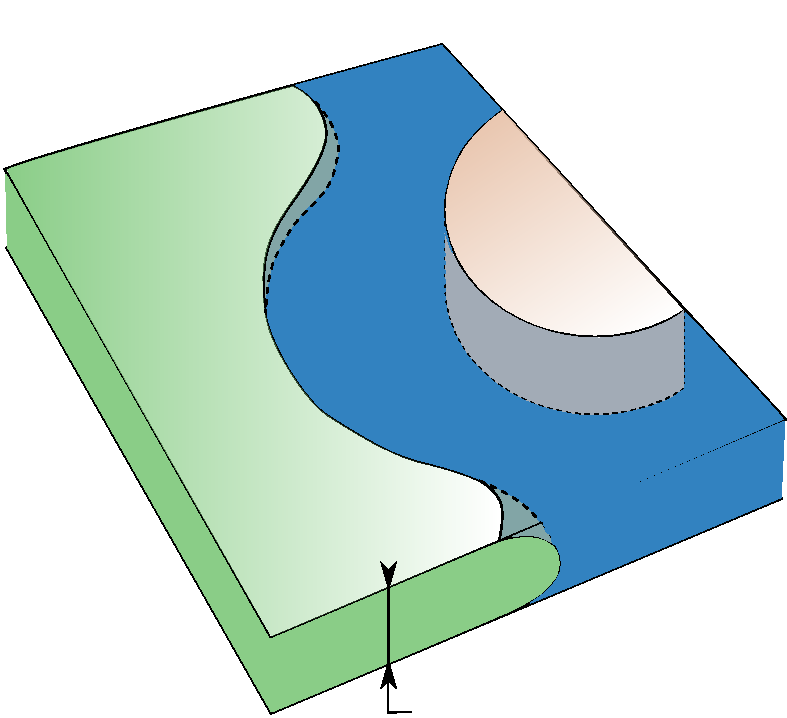
\includegraphics[width=\unitlength,page=1]{dessin_courbure.pdf}}%
    \put(0.52814239,0.00000007){\color[rgb]{0,0,0}\makebox(0,0)[lt]{\lineheight{1.25}\smash{\begin{tabular}[t]{l}$h$\end{tabular}}}}%
    \put(0,0){\includegraphics[width=\unitlength,page=2]{dessin_courbure.pdf}}%
    \put(0.89851683,0.60307315){\color[rgb]{0,0,0}\makebox(0,0)[lt]{\lineheight{1.25}\smash{\begin{tabular}[t]{l}$A_{ws}$\end{tabular}}}}%
    \put(0.38600897,0.45714493){\color[rgb]{0,0,0}\makebox(0,0)[lt]{\lineheight{1.25}\smash{\begin{tabular}[t]{l}Fluid $w$\end{tabular}}}}%
    \put(0.11535484,0.54688159){\color[rgb]{0,0,0}\makebox(0,0)[lt]{\lineheight{1.25}\smash{\begin{tabular}[t]{l}Fluid $o$\end{tabular}}}}%
    \put(0,0){\includegraphics[width=\unitlength,page=3]{dessin_courbure.pdf}}%
    \put(0.83936721,0.14449571){\color[rgb]{0,0,0}\makebox(0,0)[lt]{\lineheight{1.25}\smash{\begin{tabular}[t]{l}$A_{wo}$\end{tabular}}}}%
    \put(0,0){\includegraphics[width=\unitlength,page=4]{dessin_courbure.pdf}}%
    \put(0.2590285,0.8342462){\color[rgb]{0,0,0}\makebox(0,0)[lt]{\lineheight{1.25}\smash{\begin{tabular}[t]{l}$l$\end{tabular}}}}%
    \put(0,0){\includegraphics[width=\unitlength,page=5]{dessin_courbure.pdf}}%
    \put(0.75698471,0.73356527){\color[rgb]{0,0,0}\makebox(0,0)[lt]{\lineheight{1.25}\smash{\begin{tabular}[t]{l}$x$\end{tabular}}}}%
    \put(0.93038067,0.70236227){\color[rgb]{0,0,0}\makebox(0,0)[lt]{\lineheight{1.25}\smash{\begin{tabular}[t]{l}$y$\end{tabular}}}}%
    \put(0.85428739,0.79145817){\color[rgb]{0,0,0}\makebox(0,0)[lt]{\lineheight{1.25}\smash{\begin{tabular}[t]{l}$z$\end{tabular}}}}%
    \put(0,0){\includegraphics[width=\unitlength,page=6]{dessin_courbure.pdf}}%
  \end{picture}%
\endgroup%

\par\end{centering}
\caption{Illustation of confined cocurrent two-phase flow between two parallel
plates and around cylinder obstacles.\label{fig:modelHeleShaw}}
\end{figure}

To compute the traction exerted by the fluids upon the cell plates
we consider that the flow velocity is only oriented with the $x$-axis
and that it depends only on the $z$-coordinate, where its profile
follows the Poiseuille's law,

\[
u=-\frac{1}{2\mu}\frac{dp}{dx}z(z-h).
\]

Then the friction force exerted on the bottom plate is given by

\[
\mu\frac{\partial u}{\partial z}\mid_{z=0}=-\frac{h}{2}\frac{dp}{dx}.
\]

Thus, the traction $T_{i,pl}^{x}$ is obtained by multiplying the
friction force by two times the surface wetted by the fluid $i$.

Going beyond the approximation that the velocity depends only on the
$z$-coordinates we note that the average velocity taken over the
interval between the plates is written as follows 

\[
\mathbf{U}(x,y,0)=-\frac{h^{2}}{12\mu}\nabla_{\parallel}p.
\]

There is therefore a direct analogy between the flow in a 2D porous
medium and the flow in a Hele-Shaw cell for which the permeability
is given by $h^{2}/12$ \citep{saffman1958penetration}. This allows
us in the following to modify the absolute permeability of the structure
without modifying its overall geometry, just by varying the aperture
between the plates.

Beside the interface curvature in the Hele-Shaw cell plane, the meniscus
in the perpendicular plane must be taken into account. Considering
it as a semicircle of radius $h/2$, the pressure jump at equilibrium
across the interface reads

\begin{equation}
\Delta p=\gamma\left(\frac{2}{h}+\kappa_{\parallel}\right),\label{eq:curvatureHeleShaw}
\end{equation}

where $\gamma$ denotes the surface tension and $\kappa_{\parallel}$
the curvature in the Hele-Shaw plane. Eq.~\ref{eq:curvatureHeleShaw}
was completed by \citet{park1984two} with an additional term that
pertains for dynamic film formation and a corrective $\pi/4$ factor
for the curvature in the cell plane. The reader is warnes that while
dynamic film formation along the plates is an important phenomenom
regarding the flow \citep{jackson2015dynamic}, this question requires
dedicated study and is beyond the scope of this article. Thus, we
consider in the following that the invading fluid is in contact with
the cell plates, i.e. presence of a triple line.-


\section{Direct numerical simulations\label{sec:Direct-numerical-simulations}}

\subsection{Equations}

\subsubsection{Level Set model}

We used the standard Level Set method to capture the moving free interface
between the fluids. The method is part of Eulerian methods which have
the particularity of easily reproducing topological changes of the
phases contrary to Lagrangian methods. As topological changes of the
fluids is not excluded here, this motivated the choice for this type
of method. In this framework the fluid phases are identified with
a level set (scalar) function that goes smoothly from 0 to 1 across
the fluid interface, which is implicitely defined as the iso-level
$\phi=0.5$. Transport of the level set function $\phi$ is governed
by

\begin{equation}
\frac{\partial\phi}{\partial t}+\nabla\cdot(\mathbf{u}\phi)=\tau\nabla\cdot\left(\psi\boldsymbol{\nabla}\phi-\phi(1-\phi)\frac{\boldsymbol{\nabla}\phi}{\vert\nabla\phi\vert}\right).\label{eq:advecPhi}
\end{equation}

In this equation, $\mathbf{u}$ is the velocity field and $\tau$
and $\psi$ are two numerical parameters that control the diffuse
interface thickness and the amount of reinitialization of $\phi$
function, respectively \citep{Olsson2007}. 

\subsubsection{Flow equations}

Remember that we need to take into account tangential stress as well
perpendicular stress due to flow confinement, a full-3D resolution
of flow equations would be meaningful. In order to avoid solving such
resource-intensive simulations we rather resolved 2D flow equations
plus an additional term taking into account the perpendicular stress.
Velocity and pressure fields are obtained by solving 2D-modified Stokes
equations since the Reynolds number is assumed to be sufficiently
low so that the flow is creeping. The whole-domain formulation Stokes
and continuity equations read

\begin{subequations}

\begin{equation}
0=-\nabla p+\mu(\phi)\left(\nabla^{2}\mathbf{u}-k^{2}\mathbf{u}\right)+\mathbf{F}_{st},
\end{equation}

\begin{equation}
0=\nabla\cdot\mathbf{u},
\end{equation}

\end{subequations}

where $k=\frac{\sqrt{12}}{h}$ is an additional term that pertain
to a Darcy-term arising from depth-averaging of Stokes equation, as
described in the theoretical background section and $\mathbf{F}_{st}$
is the surface tension fore per unit volume. This term is defined
here as a purely normal contribution, i.e. constant surface tension
along the interface, and reads

\[
\mathbf{F}_{st}=\gamma\kappa\delta(\phi)\mathbf{n},
\]

where $\mathbf{n}$ denotes the unit normal to the interface and $\delta(\phi)$
is the Dirac delta function localized on the interface \citep{Sussman1994}.
In this framework the unit normal vector as well as the mean curvature
are obtained with the level set function $\phi$ as 

\begin{equation}
\mathbf{n}=\frac{\boldsymbol{\nabla}\phi}{\vert\boldsymbol{\nabla}\phi\vert},
\end{equation}

\begin{equation}
\kappa=\frac{\pi}{4}\nabla\cdot\left(\frac{\boldsymbol{\nabla}\phi}{\vert\boldsymbol{\nabla}\phi\vert}\right)+\frac{2}{h},
\end{equation}

respectively, where we added the $\pi/4$ factor in the curvature
expression to be consistent with the correction derived by \citet{park1984two}.

The fluid density and the fluid viscosity vary smoothly from one fluid
to another 

\[
\rho(\phi)=\rho_{o}+(\rho_{w}-\rho_{o})\phi,
\]

\[
\mu(\phi)=\mu_{o}+(\mu_{w}-\mu_{o})\phi.
\]


\subsubsection{Dimensionless equations and relevant dimensionless numbers}

If one define the following dimensionless variables

\[
\mathbf{u}=\mathbf{u}'\times U,\;p=p'\times\frac{\mu U}{l},\;\kappa=\kappa'\times l,\;\mathbf{x}=\mathbf{x}'\times l,
\]

where $U$ is a reference velocity, $\mu$ a reference viscosity and
$l$ a reference length, Stokes and continuity equations can be recast
as

\[
0=-\nabla'p'+\frac{\mu(\phi)}{\mu}\nabla'^{2}\mathbf{u}'+\frac{\gamma}{\mu U}\kappa'\nabla'\phi,
\]

\[
0=\nabla'\cdot\mathbf{u}'.
\]

One can notice the two following dimensionless numbers

\[
\bar{\mu}=\frac{\mu(\phi)}{\mu},\;Ca^{-1}=\frac{\gamma}{\mu U},
\]

the viscosity ratio and the capillary number, respectively, which
add up to the aspect ratio $h/l$.

In the following, the results are given as a function of 

\[
Ca=\frac{(U_{o}+U_{w})\mu_{o}}{\gamma},\qquad U_{w}^{'}=\frac{U_{w}}{U_{o}+U_{w}}=f_{f},\qquad U_{o}^{'}=1-f_{f},
\]

where $f_{f}$ is called fractional flow, the reference viscosity
is the invading fluid viscosity ($\mu_{o}=2\times\mu_{w}=2\times10^{-3}$
Pa.s) and the reference velocity is the total velocity $U=U_{o}+U_{w}$.
The viscosity ratio $\bar{\mu}$ as well as the fractional flow $f_{f}$
are kept constant at 2 and 0.25, respectively, and the reference length
is the cell's width denoted $l=5\times10^{-4}$ m . 

\subsection{Geometry and boundary conditions}

We study a model system consisting of an array of cylinders in a thin
square cuboid, resembling a Hele-Shaw-cell with obstacles, as shown
in Fig.~\ref{fig:model}. The two fluids are injected from the left
at a constant normal velocity. The outlet boundary condition for the
flow is a constant pressure. Initially the wetting fluid occupy the
entire geometry. The different boundary conditions are listed in \ref{tab:Boundary-conditions}.

\begin{figure}
\begin{centering}
%% Creator: Inkscape inkscape 0.92.4, www.inkscape.org
%% PDF/EPS/PS + LaTeX output extension by Johan Engelen, 2010
%% Accompanies image file 'model.pdf' (pdf, eps, ps)
%%
%% To include the image in your LaTeX document, write
%%   \input{<filename>.pdf_tex}
%%  instead of
%%   \includegraphics{<filename>.pdf}
%% To scale the image, write
%%   \def\svgwidth{<desired width>}
%%   \input{<filename>.pdf_tex}
%%  instead of
%%   \includegraphics[width=<desired width>]{<filename>.pdf}
%%
%% Images with a different path to the parent latex file can
%% be accessed with the `import' package (which may need to be
%% installed) using
%%   \usepackage{import}
%% in the preamble, and then including the image with
%%   \import{<path to file>}{<filename>.pdf_tex}
%% Alternatively, one can specify
%%   \graphicspath{{<path to file>/}}
%% 
%% For more information, please see info/svg-inkscape on CTAN:
%%   http://tug.ctan.org/tex-archive/info/svg-inkscape
%%
\begingroup%
  \makeatletter%
  \providecommand\color[2][]{%
    \errmessage{(Inkscape) Color is used for the text in Inkscape, but the package 'color.sty' is not loaded}%
    \renewcommand\color[2][]{}%
  }%
  \providecommand\transparent[1]{%
    \errmessage{(Inkscape) Transparency is used (non-zero) for the text in Inkscape, but the package 'transparent.sty' is not loaded}%
    \renewcommand\transparent[1]{}%
  }%
  \providecommand\rotatebox[2]{#2}%
  \newcommand*\fsize{\dimexpr\f@size pt\relax}%
  \newcommand*\lineheight[1]{\fontsize{\fsize}{#1\fsize}\selectfont}%
  \ifx\svgwidth\undefined%
    \setlength{\unitlength}{443.15460926bp}%
    \ifx\svgscale\undefined%
      \relax%
    \else%
      \setlength{\unitlength}{\unitlength * \real{\svgscale}}%
    \fi%
  \else%
    \setlength{\unitlength}{\svgwidth}%
  \fi%
  \global\let\svgwidth\undefined%
  \global\let\svgscale\undefined%
  \makeatother%
  \begin{picture}(1,0.56587843)%
    \lineheight{1}%
    \setlength\tabcolsep{0pt}%
    \put(0,0){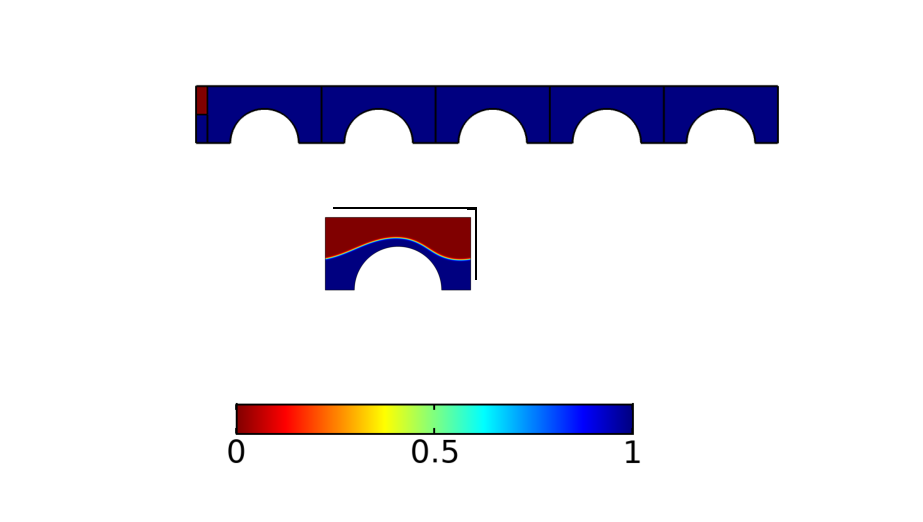
\includegraphics[width=\unitlength,page=1]{model.pdf}}%
    \put(0.26660576,0.47767245){\color[rgb]{0,0,0}\makebox(0,0)[lt]{\lineheight{1.25}\smash{\begin{tabular}[t]{l}UC1\end{tabular}}}}%
    \put(0.3869981,0.47767245){\color[rgb]{0,0,0}\makebox(0,0)[lt]{\lineheight{1.25}\smash{\begin{tabular}[t]{l}UC2\end{tabular}}}}%
    \put(0.51077273,0.47767245){\color[rgb]{0,0,0}\makebox(0,0)[lt]{\lineheight{1.25}\smash{\begin{tabular}[t]{l}UC3\end{tabular}}}}%
    \put(0.63597003,0.47767245){\color[rgb]{0,0,0}\makebox(0,0)[lt]{\lineheight{1.25}\smash{\begin{tabular}[t]{l}UC4\end{tabular}}}}%
    \put(0.75774814,0.47767245){\color[rgb]{0,0,0}\makebox(0,0)[lt]{\lineheight{1.25}\smash{\begin{tabular}[t]{l}UC5\end{tabular}}}}%
    \put(0,0){\includegraphics[width=\unitlength,page=2]{model.pdf}}%
    \put(0.09645976,0.44349829){\color[rgb]{0,0,0}\makebox(0,0)[lt]{\lineheight{1.25}\smash{\begin{tabular}[t]{l}Inlet $o$\end{tabular}}}}%
    \put(0.09298877,0.4102802){\color[rgb]{0,0,0}\makebox(0,0)[lt]{\lineheight{1.25}\smash{\begin{tabular}[t]{l}Inlet $w$\end{tabular}}}}%
    \put(0,0){\includegraphics[width=\unitlength,page=3]{model.pdf}}%
    \put(0.8619084,0.3923161){\color[rgb]{0,0,0}\makebox(0,0)[lt]{\lineheight{1.25}\smash{\begin{tabular}[t]{l}Outlet\end{tabular}}}}%
    \put(0,0){\includegraphics[width=\unitlength,page=4]{model.pdf}}%
    \put(0.30230707,0.50596373){\color[rgb]{0,0,0}\makebox(0,0)[lt]{\lineheight{1.25}\smash{\begin{tabular}[t]{l}Symmetry\end{tabular}}}}%
    \put(0,0){\includegraphics[width=\unitlength,page=5]{model.pdf}}%
    \put(0.66206543,0.34010743){\color[rgb]{0,0,0}\makebox(0,0)[lt]{\lineheight{1.25}\smash{\begin{tabular}[t]{l}Symmetry\end{tabular}}}}%
    \put(0.22252169,0.26704458){\color[rgb]{0,0,0}\makebox(0,0)[lt]{\lineheight{1.25}\smash{\begin{tabular}[t]{l}$w$-phase\end{tabular}}}}%
    \put(0.23029302,0.30197361){\color[rgb]{0,0,0}\makebox(0,0)[lt]{\lineheight{1.25}\smash{\begin{tabular}[t]{l}$o$-phase\end{tabular}}}}%
    \put(0,0){\includegraphics[width=\unitlength,page=6]{model.pdf}}%
    \put(0.48064022,0.36146904){\color[rgb]{0,0,0}\makebox(0,0)[lt]{\lineheight{1.25}\smash{\begin{tabular}[t]{l}$h$\end{tabular}}}}%
    \put(0,0){\includegraphics[width=\unitlength,page=7]{model.pdf}}%
    \put(0.41423405,0.23059471){\color[rgb]{0,0,0}\makebox(0,0)[lt]{\lineheight{1.25}\smash{\begin{tabular}[t]{l}$A_{ws}$\end{tabular}}}}%
    \put(0,0){\includegraphics[width=\unitlength,page=8]{model.pdf}}%
    \put(0.52145744,0.22080229){\color[rgb]{0,0,0}\makebox(0,0)[lt]{\lineheight{1.25}\smash{\begin{tabular}[t]{l}$A_{wo}$\end{tabular}}}}%
    \put(0,0){\includegraphics[width=\unitlength,page=9]{model.pdf}}%
    \put(0.52647077,0.29650035){\color[rgb]{0,0,0}\rotatebox{-179.3987}{\makebox(0,0)[lt]{\lineheight{1.25}\smash{\begin{tabular}[t]{l}$l$\\\end{tabular}}}}}%
    \put(0.37233056,0.14264612){\color[rgb]{0,0,0}\makebox(0,0)[lt]{\lineheight{1.25}\smash{\begin{tabular}[t]{l}Volume fraction\end{tabular}}}}%
  \end{picture}%
\endgroup%

\par\end{centering}
\caption{The geometry used is an array of 5 cylinders in a thin square cuboid,
resembling a Hele-Shaw-cell where both fluids are injecting from left
to right, initially the square cuboïd are saturated with wetting fluid
(in blue), the length of one cell (UC) is one millimetre.\label{fig:model}}
\end{figure}

\begin{table}
\begin{centering}
\begin{tabular}{cccc}
\toprule 
Boundary & $\mathbf{u}$ & $p$ & $\ensuremath{\phi}$\tabularnewline
\midrule
\midrule 
$A_{ws}$ & 0 & - & $\mathbf{n}\cdot\mathbf{u}\phi=0$\tabularnewline
\midrule 
Outlet & - & 0 & $\mathbf{n}\cdot\boldsymbol{\nabla}\phi=0$\tabularnewline
\midrule 
Inlet $o$ & $U_{o}^{x}=\mathrm{cst}$ & - & 0\tabularnewline
\midrule 
Inlet $w$ & $U_{w}^{x}=\mathrm{cst}$ & - & 1\tabularnewline
\bottomrule
\end{tabular}
\par\end{centering}
\caption{Boundary conditions\label{tab:Boundary-conditions}}
\end{table}


\section{Results\label{sec:Results}}

Before we turn to the study of traction terms, we computed the absolute
permeability of our model, remember that it is expected to be smaller
than the $12/h^{2}$ value since the sandwiched cylinders contribute
to the pressure drop along with the cell's plates. The absolute permeability
of the model is varied by modifying the aperture between the two plates.
We used five different values for the aperture and the correspondence
in terms of absolute permeability, obtained from single-phase simulations,
is given in Tab.~\ref{tab:permeability}. When $l/h\rightarrow\infty$,
it is expected that the absolute permeability tends towards the permeability
obtained for purely 2D flow, this is observed here since the absolute
permeability for pure 2D case is $1.54\times10^{-4}$ darcy which
is very close to what we obtained for the largest aperture $h=2.5\times10^{-3}$
m. Thus, the range of absolute permeability values is typical of what
is encountered for high permeability porous media. 

\begin{table}
\caption{Equivalence between the value of the cell plates aperture and the
absolute permeability of the model obtained either from the $12/h^{2}$
value for flow between two plates or from single-phase simulation.\label{tab:permeability}}

\centering{}%
\begin{tabular}{ccc}
\toprule 
$h^{*}=h/l$ & $h^{2}/12$ (darcy) & $K$ (darcy)\tabularnewline
\midrule
\midrule 
5 & $5.2\times10^{5}$ & $1.5\times10^{4}$\tabularnewline
\midrule 
0.5 & $5.2\times10^{3}$ & $2.8\times10^{3}$\tabularnewline
\midrule 
0.25 & $1.3\times10^{3}$ & $8.6\times10^{2}$\tabularnewline
\midrule 
0.125 & $3.3\times10^{2}$ & $2.3\times10^{2}$\tabularnewline
\midrule 
0.05 & $5.2\times10^{1}$ & $3.9\times10^{1}$\tabularnewline
\bottomrule
\end{tabular}
\end{table}

For the selected parameters, $f_{f}=0.25$ and $0.05<h^{*}<5$, we
observed only a film-flow regime without any phase rupture. The wetting
fluid saturation in one cuboid, the third one in the rest of the paper
unless otherwise specified, as a function of the dimensionless aperture
and for different capillary numbers is given in Fig.~\ref{fig:Saturation}
along with corresponding selected $\phi$-fields. Wetting fluid saturation
varies between 0.3 and 0.6 and increases as the aperture increases.
The capillary number also impacts saturation by promoting the hold-up
of the wetting fluid. As seen in the selected $\phi$-fields, the
smaller the capillary the flatter the interface. For a wetting fluid
layer thickness equivalent at the plumb end of the cylinder, the saturation
is logically higher. 

\begin{figure}
\begin{centering}
% GNUPLOT: LaTeX picture with Postscript
\begingroup
  \makeatletter
  \providecommand\color[2][]{%
    \GenericError{(gnuplot) \space\space\space\@spaces}{%
      Package color not loaded in conjunction with
      terminal option `colourtext'%
    }{See the gnuplot documentation for explanation.%
    }{Either use 'blacktext' in gnuplot or load the package
      color.sty in LaTeX.}%
    \renewcommand\color[2][]{}%
  }%
  \providecommand\includegraphics[2][]{%
    \GenericError{(gnuplot) \space\space\space\@spaces}{%
      Package graphicx or graphics not loaded%
    }{See the gnuplot documentation for explanation.%
    }{The gnuplot epslatex terminal needs graphicx.sty or graphics.sty.}%
    \renewcommand\includegraphics[2][]{}%
  }%
  \providecommand\rotatebox[2]{#2}%
  \@ifundefined{ifGPcolor}{%
    \newif\ifGPcolor
    \GPcolortrue
  }{}%
  \@ifundefined{ifGPblacktext}{%
    \newif\ifGPblacktext
    \GPblacktexttrue
  }{}%
  % define a \g@addto@macro without @ in the name:
  \let\gplgaddtomacro\g@addto@macro
  % define empty templates for all commands taking text:
  \gdef\gplbacktext{}%
  \gdef\gplfronttext{}%
  \makeatother
  \ifGPblacktext
    % no textcolor at all
    \def\colorrgb#1{}%
    \def\colorgray#1{}%
  \else
    % gray or color?
    \ifGPcolor
      \def\colorrgb#1{\color[rgb]{#1}}%
      \def\colorgray#1{\color[gray]{#1}}%
      \expandafter\def\csname LTw\endcsname{\color{white}}%
      \expandafter\def\csname LTb\endcsname{\color{black}}%
      \expandafter\def\csname LTa\endcsname{\color{black}}%
      \expandafter\def\csname LT0\endcsname{\color[rgb]{1,0,0}}%
      \expandafter\def\csname LT1\endcsname{\color[rgb]{0,1,0}}%
      \expandafter\def\csname LT2\endcsname{\color[rgb]{0,0,1}}%
      \expandafter\def\csname LT3\endcsname{\color[rgb]{1,0,1}}%
      \expandafter\def\csname LT4\endcsname{\color[rgb]{0,1,1}}%
      \expandafter\def\csname LT5\endcsname{\color[rgb]{1,1,0}}%
      \expandafter\def\csname LT6\endcsname{\color[rgb]{0,0,0}}%
      \expandafter\def\csname LT7\endcsname{\color[rgb]{1,0.3,0}}%
      \expandafter\def\csname LT8\endcsname{\color[rgb]{0.5,0.5,0.5}}%
    \else
      % gray
      \def\colorrgb#1{\color{black}}%
      \def\colorgray#1{\color[gray]{#1}}%
      \expandafter\def\csname LTw\endcsname{\color{white}}%
      \expandafter\def\csname LTb\endcsname{\color{black}}%
      \expandafter\def\csname LTa\endcsname{\color{black}}%
      \expandafter\def\csname LT0\endcsname{\color{black}}%
      \expandafter\def\csname LT1\endcsname{\color{black}}%
      \expandafter\def\csname LT2\endcsname{\color{black}}%
      \expandafter\def\csname LT3\endcsname{\color{black}}%
      \expandafter\def\csname LT4\endcsname{\color{black}}%
      \expandafter\def\csname LT5\endcsname{\color{black}}%
      \expandafter\def\csname LT6\endcsname{\color{black}}%
      \expandafter\def\csname LT7\endcsname{\color{black}}%
      \expandafter\def\csname LT8\endcsname{\color{black}}%
    \fi
  \fi
    \setlength{\unitlength}{0.0500bp}%
    \ifx\gptboxheight\undefined%
      \newlength{\gptboxheight}%
      \newlength{\gptboxwidth}%
      \newsavebox{\gptboxtext}%
    \fi%
    \setlength{\fboxrule}{0.5pt}%
    \setlength{\fboxsep}{1pt}%
\begin{picture}(7200.00,4320.00)%
    \gplgaddtomacro\gplbacktext{%
      \colorrgb{0.50,0.50,0.50}%%
      \put(1949,595){\makebox(0,0)[r]{\strut{}$0$}}%
      \colorrgb{0.50,0.50,0.50}%%
      \put(1949,1303){\makebox(0,0)[r]{\strut{}$0.2$}}%
      \colorrgb{0.50,0.50,0.50}%%
      \put(1949,2010){\makebox(0,0)[r]{\strut{}$0.4$}}%
      \colorrgb{0.50,0.50,0.50}%%
      \put(1949,2718){\makebox(0,0)[r]{\strut{}$0.6$}}%
      \colorrgb{0.50,0.50,0.50}%%
      \put(1949,3425){\makebox(0,0)[r]{\strut{}$0.8$}}%
      \colorrgb{0.50,0.50,0.50}%%
      \put(1949,4133){\makebox(0,0)[r]{\strut{}$1$}}%
      \colorrgb{0.50,0.50,0.50}%%
      \put(2051,409){\makebox(0,0){\strut{}$0.1$}}%
      \colorrgb{0.50,0.50,0.50}%%
      \put(3526,409){\makebox(0,0){\strut{}$1$}}%
      \colorrgb{0.50,0.50,0.50}%%
      \put(5002,409){\makebox(0,0){\strut{}$10$}}%
    }%
    \gplgaddtomacro\gplfronttext{%
      \csname LTb\endcsname%%
      \put(1457,2364){\rotatebox{-270}{\makebox(0,0){\strut{}$S_w$}}}%
      \csname LTb\endcsname%%
      \put(3820,130){\makebox(0,0){\strut{}$1/h^*$}}%
      \csname LTb\endcsname%%
      \put(4801,3919){\makebox(0,0)[r]{\strut{}$Ca=1.0 \times 10^{0}$}}%
      \csname LTb\endcsname%%
      \put(4801,3640){\makebox(0,0)[r]{\strut{}$Ca=5.0 \times 10^{-2}$}}%
      \csname LTb\endcsname%%
      \put(4801,3361){\makebox(0,0)[r]{\strut{}$Ca=7.5 \times 10^{-3}$}}%
    }%
    \gplbacktext
    \put(0,0){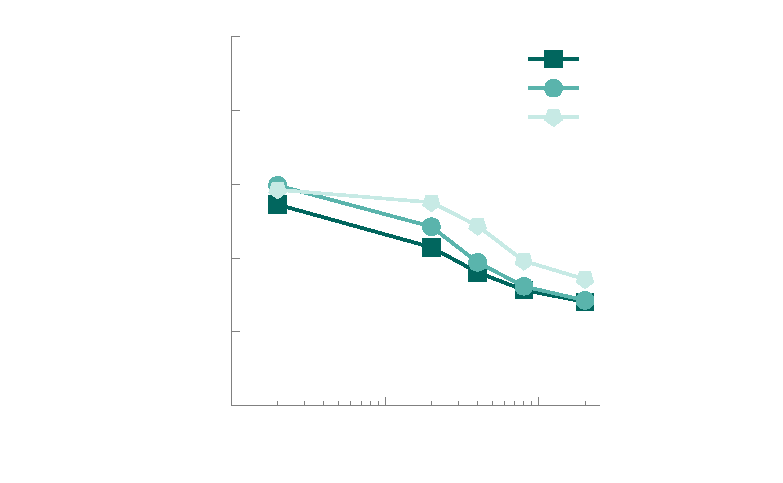
\includegraphics{saturation}}%
    \gplfronttext
  \end{picture}%
\endgroup

\par\end{centering}
\caption{Wetting fluid saturation in UC3 as a function of the dimensionless
aperture between the Hele-Shaw plates and for different capillary
numbers at steasy-state\label{fig:Saturation}}

\end{figure}

Let us now take a closer look at the dynamic capillary pressure as
expressed in Eq.~ and the pressure fields. Here, as can be seen in
Fig.~\ref{fig:Pc}, the difference in intrinsic mean pressure of
the fluids is entirely controlled by the pressure jump caused by the
out-of-plane meniscus, even for the larger aperture, and does not
depends on the capillary number at all. How the pressure jump compared
to the pressure gradient across a cell? Based on the pressure fields
in Fig.~\ref{fig:pField} one can answer that for $Ca=1$ the pressure
gradient across the cell is larger than the pressure jump and, interestingly,
it becomes larger and larger than the pressure jump as the aperture
between the plates is reduced. It is quite different when the capillary
number decreases, and for $Ca=0.01$ combined with a large aperture
the pressure gradient across the cell is negligible in front of the
pressure jump due to surface tension effects. As the aperture decreases,
the pressure gradient increases and becomes comparable to the pressure
jump, but the pressure itsel is differently distributed in the cell
compared to higher capillary number cases with a higher pressure in
the wetting fluid. 

\begin{figure}
\begin{centering}
% GNUPLOT: LaTeX picture with Postscript
\begingroup
  % Encoding inside the plot.  In the header of your document, this encoding
  % should to defined, e.g., by using
  % \usepackage[cp1252,<other encodings>]{inputenc}
  \makeatletter
  \providecommand\color[2][]{%
    \GenericError{(gnuplot) \space\space\space\@spaces}{%
      Package color not loaded in conjunction with
      terminal option `colourtext'%
    }{See the gnuplot documentation for explanation.%
    }{Either use 'blacktext' in gnuplot or load the package
      color.sty in LaTeX.}%
    \renewcommand\color[2][]{}%
  }%
  \providecommand\includegraphics[2][]{%
    \GenericError{(gnuplot) \space\space\space\@spaces}{%
      Package graphicx or graphics not loaded%
    }{See the gnuplot documentation for explanation.%
    }{The gnuplot epslatex terminal needs graphicx.sty or graphics.sty.}%
    \renewcommand\includegraphics[2][]{}%
  }%
  \providecommand\rotatebox[2]{#2}%
  \@ifundefined{ifGPcolor}{%
    \newif\ifGPcolor
    \GPcolortrue
  }{}%
  \@ifundefined{ifGPblacktext}{%
    \newif\ifGPblacktext
    \GPblacktexttrue
  }{}%
  % define a \g@addto@macro without @ in the name:
  \let\gplgaddtomacro\g@addto@macro
  % define empty templates for all commands taking text:
  \gdef\gplbacktext{}%
  \gdef\gplfronttext{}%
  \makeatother
  \ifGPblacktext
    % no textcolor at all
    \def\colorrgb#1{}%
    \def\colorgray#1{}%
  \else
    % gray or color?
    \ifGPcolor
      \def\colorrgb#1{\color[rgb]{#1}}%
      \def\colorgray#1{\color[gray]{#1}}%
      \expandafter\def\csname LTw\endcsname{\color{white}}%
      \expandafter\def\csname LTb\endcsname{\color{black}}%
      \expandafter\def\csname LTa\endcsname{\color{black}}%
      \expandafter\def\csname LT0\endcsname{\color[rgb]{1,0,0}}%
      \expandafter\def\csname LT1\endcsname{\color[rgb]{0,1,0}}%
      \expandafter\def\csname LT2\endcsname{\color[rgb]{0,0,1}}%
      \expandafter\def\csname LT3\endcsname{\color[rgb]{1,0,1}}%
      \expandafter\def\csname LT4\endcsname{\color[rgb]{0,1,1}}%
      \expandafter\def\csname LT5\endcsname{\color[rgb]{1,1,0}}%
      \expandafter\def\csname LT6\endcsname{\color[rgb]{0,0,0}}%
      \expandafter\def\csname LT7\endcsname{\color[rgb]{1,0.3,0}}%
      \expandafter\def\csname LT8\endcsname{\color[rgb]{0.5,0.5,0.5}}%
    \else
      % gray
      \def\colorrgb#1{\color{black}}%
      \def\colorgray#1{\color[gray]{#1}}%
      \expandafter\def\csname LTw\endcsname{\color{white}}%
      \expandafter\def\csname LTb\endcsname{\color{black}}%
      \expandafter\def\csname LTa\endcsname{\color{black}}%
      \expandafter\def\csname LT0\endcsname{\color{black}}%
      \expandafter\def\csname LT1\endcsname{\color{black}}%
      \expandafter\def\csname LT2\endcsname{\color{black}}%
      \expandafter\def\csname LT3\endcsname{\color{black}}%
      \expandafter\def\csname LT4\endcsname{\color{black}}%
      \expandafter\def\csname LT5\endcsname{\color{black}}%
      \expandafter\def\csname LT6\endcsname{\color{black}}%
      \expandafter\def\csname LT7\endcsname{\color{black}}%
      \expandafter\def\csname LT8\endcsname{\color{black}}%
    \fi
  \fi
    \setlength{\unitlength}{0.0500bp}%
    \ifx\gptboxheight\undefined%
      \newlength{\gptboxheight}%
      \newlength{\gptboxwidth}%
      \newsavebox{\gptboxtext}%
    \fi%
    \setlength{\fboxrule}{0.5pt}%
    \setlength{\fboxsep}{1pt}%
\begin{picture}(7180.00,4300.00)%
    \gplgaddtomacro\gplbacktext{%
      \colorrgb{0.50,0.50,0.50}%%
      \put(849,700){\makebox(0,0)[r]{\strut{}$0.001$}}%
      \colorrgb{0.50,0.50,0.50}%%
      \put(849,1827){\makebox(0,0)[r]{\strut{}$0.01$}}%
      \colorrgb{0.50,0.50,0.50}%%
      \put(849,2953){\makebox(0,0)[r]{\strut{}$0.1$}}%
      \colorrgb{0.50,0.50,0.50}%%
      \put(849,4080){\makebox(0,0)[r]{\strut{}$1$}}%
      \colorrgb{0.50,0.50,0.50}%%
      \put(2178,481){\makebox(0,0){\strut{}$0.1$}}%
      \colorrgb{0.50,0.50,0.50}%%
      \put(4533,481){\makebox(0,0){\strut{}$1$}}%
      \colorrgb{0.50,0.50,0.50}%%
      \put(6888,481){\makebox(0,0){\strut{}$10$}}%
    }%
    \gplgaddtomacro\gplfronttext{%
      \csname LTb\endcsname%%
      \put(182,2390){\rotatebox{-270}{\makebox(0,0){\strut{}$\vert P_o-P_w\:(\mathrm{Pa}) \vert$}}}%
      \csname LTb\endcsname%%
      \put(3917,153){\makebox(0,0){\strut{}$h^*$}}%
      \csname LTb\endcsname%%
      \put(2927,1663){\makebox(0,0)[r]{\strut{}$Ca=1 \times 10^{0}$}}%
      \csname LTb\endcsname%%
      \put(2927,1335){\makebox(0,0)[r]{\strut{}$Ca=7.5 \times 10^{-3}$}}%
      \csname LTb\endcsname%%
      \put(2927,1007){\makebox(0,0)[r]{\strut{}$2\gamma/h$}}%
    }%
    \gplbacktext
    \put(0,0){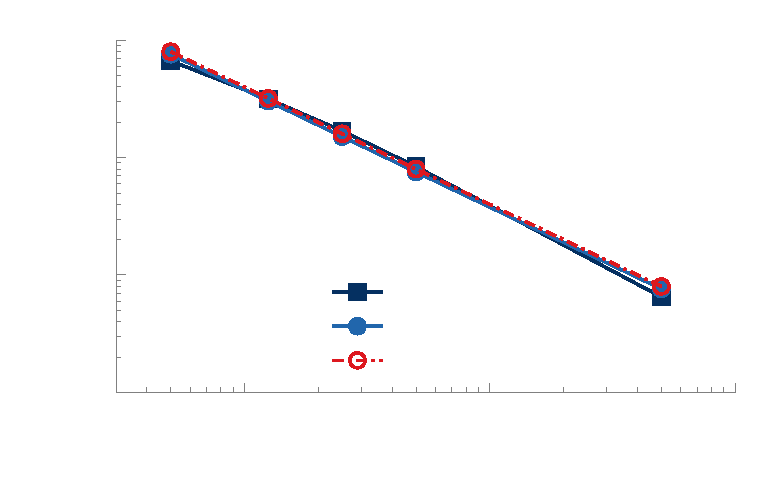
\includegraphics{Pc}}%
    \gplfronttext
  \end{picture}%
\endgroup

\par\end{centering}
\caption{Dynamic capillary pressure in UC3 as a function of the dimensionless
aperture between the Hele-Shaw cell plates, for different capillary
numbers and pressure drop across the fluid-fluid from the out-of-plane
meniscus at steady-state.\label{fig:Pc}}

\end{figure}

\begin{figure}
\begin{centering}
%% Creator: Inkscape inkscape 0.92.4, www.inkscape.org
%% PDF/EPS/PS + LaTeX output extension by Johan Engelen, 2010
%% Accompanies image file 'pressureField.pdf' (pdf, eps, ps)
%%
%% To include the image in your LaTeX document, write
%%   \input{<filename>.pdf_tex}
%%  instead of
%%   \includegraphics{<filename>.pdf}
%% To scale the image, write
%%   \def\svgwidth{<desired width>}
%%   \input{<filename>.pdf_tex}
%%  instead of
%%   \includegraphics[width=<desired width>]{<filename>.pdf}
%%
%% Images with a different path to the parent latex file can
%% be accessed with the `import' package (which may need to be
%% installed) using
%%   \usepackage{import}
%% in the preamble, and then including the image with
%%   \import{<path to file>}{<filename>.pdf_tex}
%% Alternatively, one can specify
%%   \graphicspath{{<path to file>/}}
%% 
%% For more information, please see info/svg-inkscape on CTAN:
%%   http://tug.ctan.org/tex-archive/info/svg-inkscape
%%
\begingroup%
  \makeatletter%
  \providecommand\color[2][]{%
    \errmessage{(Inkscape) Color is used for the text in Inkscape, but the package 'color.sty' is not loaded}%
    \renewcommand\color[2][]{}%
  }%
  \providecommand\transparent[1]{%
    \errmessage{(Inkscape) Transparency is used (non-zero) for the text in Inkscape, but the package 'transparent.sty' is not loaded}%
    \renewcommand\transparent[1]{}%
  }%
  \providecommand\rotatebox[2]{#2}%
  \newcommand*\fsize{\dimexpr\f@size pt\relax}%
  \newcommand*\lineheight[1]{\fontsize{\fsize}{#1\fsize}\selectfont}%
  \ifx\svgwidth\undefined%
    \setlength{\unitlength}{362.95337587bp}%
    \ifx\svgscale\undefined%
      \relax%
    \else%
      \setlength{\unitlength}{\unitlength * \real{\svgscale}}%
    \fi%
  \else%
    \setlength{\unitlength}{\svgwidth}%
  \fi%
  \global\let\svgwidth\undefined%
  \global\let\svgscale\undefined%
  \makeatother%
  \begin{picture}(1,0.76371588)%
    \lineheight{1}%
    \setlength\tabcolsep{0pt}%
    \put(0,0){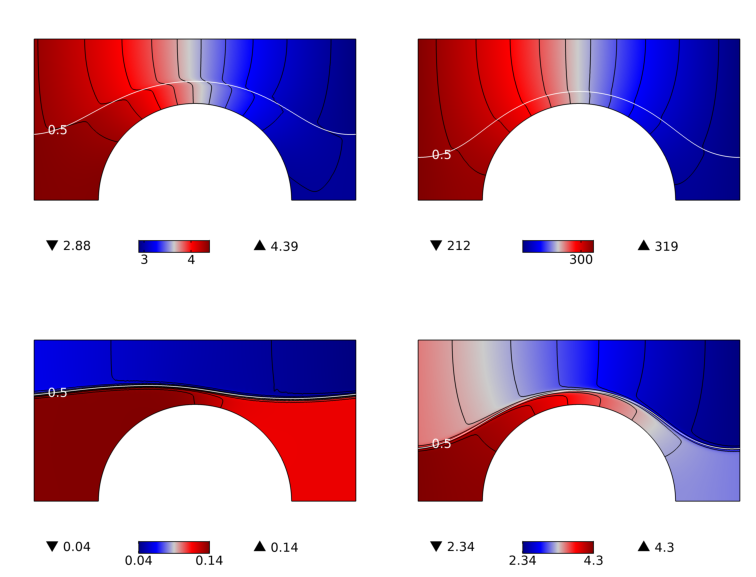
\includegraphics[width=\unitlength,page=1]{pressureField.pdf}}%
    \put(0.02120197,0.51910149){\color[rgb]{0,0,0}\rotatebox{90}{\makebox(0,0)[lt]{\lineheight{1.25}\smash{\begin{tabular}[t]{l}$Ca=1$\end{tabular}}}}}%
    \put(0.21381274,0.4585948){\color[rgb]{0,0,0}\makebox(0,0)[lt]{\lineheight{1.25}\smash{\begin{tabular}[t]{l}$p$ (Pa)\end{tabular}}}}%
    \put(0.72930006,0.45859482){\color[rgb]{0,0,0}\makebox(0,0)[lt]{\lineheight{1.25}\smash{\begin{tabular}[t]{l}$p$ (Pa)\end{tabular}}}}%
    \put(0.21325872,0.06007846){\color[rgb]{0,0,0}\makebox(0,0)[lt]{\lineheight{1.25}\smash{\begin{tabular}[t]{l}$p$ (Pa)\end{tabular}}}}%
    \put(0.7287461,0.06007851){\color[rgb]{0,0,0}\makebox(0,0)[lt]{\lineheight{1.25}\smash{\begin{tabular}[t]{l}$p$ (Pa)\end{tabular}}}}%
    \put(0.02120197,0.09759679){\color[rgb]{0,0,0}\rotatebox{90}{\makebox(0,0)[lt]{\lineheight{1.25}\smash{\begin{tabular}[t]{l}$Ca=0.01$\end{tabular}}}}}%
    \put(0.17843311,0.74251397){\color[rgb]{0,0,0}\makebox(0,0)[lt]{\lineheight{1.25}\smash{\begin{tabular}[t]{l}$h^*=0.5$\end{tabular}}}}%
    \put(0.67678373,0.74251397){\color[rgb]{0,0,0}\makebox(0,0)[lt]{\lineheight{1.25}\smash{\begin{tabular}[t]{l}$h^*=0.05$\end{tabular}}}}%
  \end{picture}%
\endgroup%

\par\end{centering}
\caption{Pressure field in UC3 for two different capillary number and two different
dimensionless apertures, interface position as the iso-$\phi$=0.5
contour (white line) and isobar (black lines)\label{fig:pField}}

\end{figure}

We now turn to the study of the traction exerted upon the solid-fluid
boundaries $\mathbf{T}_{s}$, i.e. fluid $i$ upon the plates and
wetting fluid upon the cylinder, along with the traction at the fluid-fluid
interace $\mathbf{T}_{f}$. We focus on the magnitude of the traction
exerted at the fluid-fluid interface compared to the traction exerted
upon the solid boundaries. In the following we discuss only the $x$-component
of the traction vector $T^{x}$, i.e. aligned according to the inlet
velocity. 

The traction exerted upont the plates by the fluids was obtained as
described in the theoretical backgound section. Traction on the cylinder
boundary was obtained by calculating the integral Eq.~\ref{eq:tractionIntegral}.
We computed the fluid-fluid traction $\mathbf{T}_{f}$ in two steps.
The first step concerns the viscous part of the stress tensor, which
was calculated directly from the velocity gradients available on the
interface contour. The second step concerns the pressure part, which
was obtained by applying the divergence theorem on each phase into
a cell (UC3). 

We assessed that the traction exerted on the fluid-fluid boundary
reaches between 10 and 50\% of the traction exerted upon the solid-fluid
boundaries, as can be seen in Fig.~\ref{fig:ratioTraction}, on which
we plot the ratio $T_{f}^{x}/T_{s}^{x}$ as a function of the dimensionless
aperture between the cell plates. Interestingly, the ratio varies
non-monotonically with $h$ and the maximum value is obtained for
the smallest aperture which then decreases when the aperture increases.
The capillary number accentuates the decrease of $T_{f}^{x}$ compared
to $T_{s}^{x}$ when it decreases, as can be seen in Fig.~\ref{fig:ratioTractionCa}.

\begin{figure}
\begin{centering}
% GNUPLOT: LaTeX picture with Postscript
\begingroup
  \makeatletter
  \providecommand\color[2][]{%
    \GenericError{(gnuplot) \space\space\space\@spaces}{%
      Package color not loaded in conjunction with
      terminal option `colourtext'%
    }{See the gnuplot documentation for explanation.%
    }{Either use 'blacktext' in gnuplot or load the package
      color.sty in LaTeX.}%
    \renewcommand\color[2][]{}%
  }%
  \providecommand\includegraphics[2][]{%
    \GenericError{(gnuplot) \space\space\space\@spaces}{%
      Package graphicx or graphics not loaded%
    }{See the gnuplot documentation for explanation.%
    }{The gnuplot epslatex terminal needs graphicx.sty or graphics.sty.}%
    \renewcommand\includegraphics[2][]{}%
  }%
  \providecommand\rotatebox[2]{#2}%
  \@ifundefined{ifGPcolor}{%
    \newif\ifGPcolor
    \GPcolortrue
  }{}%
  \@ifundefined{ifGPblacktext}{%
    \newif\ifGPblacktext
    \GPblacktexttrue
  }{}%
  % define a \g@addto@macro without @ in the name:
  \let\gplgaddtomacro\g@addto@macro
  % define empty templates for all commands taking text:
  \gdef\gplbacktext{}%
  \gdef\gplfronttext{}%
  \makeatother
  \ifGPblacktext
    % no textcolor at all
    \def\colorrgb#1{}%
    \def\colorgray#1{}%
  \else
    % gray or color?
    \ifGPcolor
      \def\colorrgb#1{\color[rgb]{#1}}%
      \def\colorgray#1{\color[gray]{#1}}%
      \expandafter\def\csname LTw\endcsname{\color{white}}%
      \expandafter\def\csname LTb\endcsname{\color{black}}%
      \expandafter\def\csname LTa\endcsname{\color{black}}%
      \expandafter\def\csname LT0\endcsname{\color[rgb]{1,0,0}}%
      \expandafter\def\csname LT1\endcsname{\color[rgb]{0,1,0}}%
      \expandafter\def\csname LT2\endcsname{\color[rgb]{0,0,1}}%
      \expandafter\def\csname LT3\endcsname{\color[rgb]{1,0,1}}%
      \expandafter\def\csname LT4\endcsname{\color[rgb]{0,1,1}}%
      \expandafter\def\csname LT5\endcsname{\color[rgb]{1,1,0}}%
      \expandafter\def\csname LT6\endcsname{\color[rgb]{0,0,0}}%
      \expandafter\def\csname LT7\endcsname{\color[rgb]{1,0.3,0}}%
      \expandafter\def\csname LT8\endcsname{\color[rgb]{0.5,0.5,0.5}}%
    \else
      % gray
      \def\colorrgb#1{\color{black}}%
      \def\colorgray#1{\color[gray]{#1}}%
      \expandafter\def\csname LTw\endcsname{\color{white}}%
      \expandafter\def\csname LTb\endcsname{\color{black}}%
      \expandafter\def\csname LTa\endcsname{\color{black}}%
      \expandafter\def\csname LT0\endcsname{\color{black}}%
      \expandafter\def\csname LT1\endcsname{\color{black}}%
      \expandafter\def\csname LT2\endcsname{\color{black}}%
      \expandafter\def\csname LT3\endcsname{\color{black}}%
      \expandafter\def\csname LT4\endcsname{\color{black}}%
      \expandafter\def\csname LT5\endcsname{\color{black}}%
      \expandafter\def\csname LT6\endcsname{\color{black}}%
      \expandafter\def\csname LT7\endcsname{\color{black}}%
      \expandafter\def\csname LT8\endcsname{\color{black}}%
    \fi
  \fi
    \setlength{\unitlength}{0.0500bp}%
    \ifx\gptboxheight\undefined%
      \newlength{\gptboxheight}%
      \newlength{\gptboxwidth}%
      \newsavebox{\gptboxtext}%
    \fi%
    \setlength{\fboxrule}{0.5pt}%
    \setlength{\fboxsep}{1pt}%
\begin{picture}(7200.00,4320.00)%
    \gplgaddtomacro\gplbacktext{%
      \colorrgb{0.50,0.50,0.50}%%
      \put(1949,595){\makebox(0,0)[r]{\strut{}$0$}}%
      \colorrgb{0.50,0.50,0.50}%%
      \put(1949,1303){\makebox(0,0)[r]{\strut{}$0.2$}}%
      \colorrgb{0.50,0.50,0.50}%%
      \put(1949,2010){\makebox(0,0)[r]{\strut{}$0.4$}}%
      \colorrgb{0.50,0.50,0.50}%%
      \put(1949,2718){\makebox(0,0)[r]{\strut{}$0.6$}}%
      \colorrgb{0.50,0.50,0.50}%%
      \put(1949,3425){\makebox(0,0)[r]{\strut{}$0.8$}}%
      \colorrgb{0.50,0.50,0.50}%%
      \put(1949,4133){\makebox(0,0)[r]{\strut{}$1$}}%
      \colorrgb{0.50,0.50,0.50}%%
      \put(2051,409){\makebox(0,0){\strut{}$0.1$}}%
      \colorrgb{0.50,0.50,0.50}%%
      \put(3479,409){\makebox(0,0){\strut{}$1$}}%
      \colorrgb{0.50,0.50,0.50}%%
      \put(4908,409){\makebox(0,0){\strut{}$10$}}%
    }%
    \gplgaddtomacro\gplfronttext{%
      \csname LTb\endcsname%%
      \put(1457,2364){\rotatebox{-270}{\makebox(0,0){\strut{}$T_{int}^x/T_{s}^x$}}}%
      \csname LTb\endcsname%%
      \put(3820,130){\makebox(0,0){\strut{}$1/h^*$}}%
      \csname LTb\endcsname%%
      \put(3792,3663){\makebox(0,0)[r]{\strut{}$Ca=1 \times 10^{0}$}}%
      \csname LTb\endcsname%%
      \put(3792,3431){\makebox(0,0)[r]{\strut{}$Ca=5 \times 10^{-2}$}}%
      \csname LTb\endcsname%%
      \put(3792,3199){\makebox(0,0)[r]{\strut{}$Ca=1 \times 10^{-2}$}}%
      \csname LTb\endcsname%%
      \put(3792,2967){\makebox(0,0)[r]{\strut{}$Ca=7.5 \times 10^{-3}$}}%
    }%
    \gplbacktext
    \put(0,0){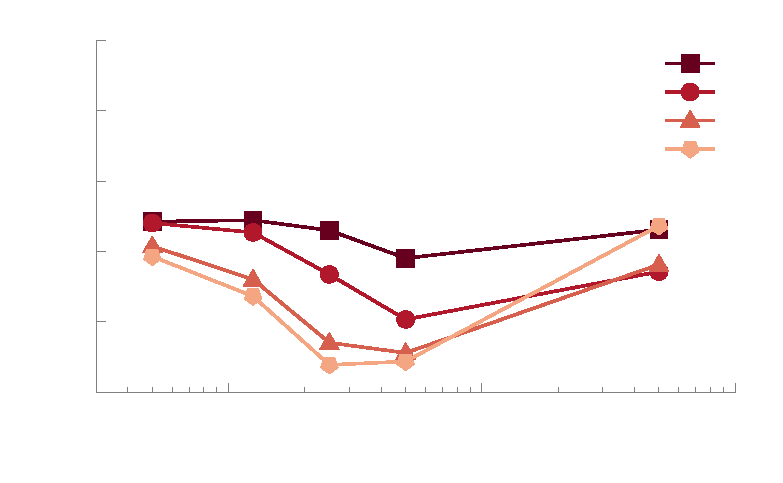
\includegraphics{ratioDrag}}%
    \gplfronttext
  \end{picture}%
\endgroup

\par\end{centering}
\caption{Ratio of traction ($x$-component) on fluid-fluid interface over traction
on solid-fluid interfaces in UC3 as a function of the dimensionless
aperture between the Hele-Shaw plates and for different capillary
numbers at steady-state.\label{fig:ratioTraction}}
\end{figure}

\begin{figure}
\begin{centering}
% GNUPLOT: LaTeX picture with Postscript
\begingroup
  % Encoding inside the plot.  In the header of your document, this encoding
  % should to defined, e.g., by using
  % \usepackage[cp1252,<other encodings>]{inputenc}

  \makeatletter
  \providecommand\color[2][]{%
    \GenericError{(gnuplot) \space\space\space\@spaces}{%
      Package color not loaded in conjunction with
      terminal option `colourtext'%
    }{See the gnuplot documentation for explanation.%
    }{Either use 'blacktext' in gnuplot or load the package
      color.sty in LaTeX.}%
    \renewcommand\color[2][]{}%
  }%
  \providecommand\includegraphics[2][]{%
    \GenericError{(gnuplot) \space\space\space\@spaces}{%
      Package graphicx or graphics not loaded%
    }{See the gnuplot documentation for explanation.%
    }{The gnuplot epslatex terminal needs graphicx.sty or graphics.sty.}%
    \renewcommand\includegraphics[2][]{}%
  }%
  \providecommand\rotatebox[2]{#2}%
  \@ifundefined{ifGPcolor}{%
    \newif\ifGPcolor
    \GPcolortrue
  }{}%
  \@ifundefined{ifGPblacktext}{%
    \newif\ifGPblacktext
    \GPblacktexttrue
  }{}%
  % define a \g@addto@macro without @ in the name:
  \let\gplgaddtomacro\g@addto@macro
  % define empty templates for all commands taking text:
  \gdef\gplbacktext{}%
  \gdef\gplfronttext{}%
  \makeatother
  \ifGPblacktext
    % no textcolor at all
    \def\colorrgb#1{}%
    \def\colorgray#1{}%
  \else
    % gray or color?
    \ifGPcolor
      \def\colorrgb#1{\color[rgb]{#1}}%
      \def\colorgray#1{\color[gray]{#1}}%
      \expandafter\def\csname LTw\endcsname{\color{white}}%
      \expandafter\def\csname LTb\endcsname{\color{black}}%
      \expandafter\def\csname LTa\endcsname{\color{black}}%
      \expandafter\def\csname LT0\endcsname{\color[rgb]{1,0,0}}%
      \expandafter\def\csname LT1\endcsname{\color[rgb]{0,1,0}}%
      \expandafter\def\csname LT2\endcsname{\color[rgb]{0,0,1}}%
      \expandafter\def\csname LT3\endcsname{\color[rgb]{1,0,1}}%
      \expandafter\def\csname LT4\endcsname{\color[rgb]{0,1,1}}%
      \expandafter\def\csname LT5\endcsname{\color[rgb]{1,1,0}}%
      \expandafter\def\csname LT6\endcsname{\color[rgb]{0,0,0}}%
      \expandafter\def\csname LT7\endcsname{\color[rgb]{1,0.3,0}}%
      \expandafter\def\csname LT8\endcsname{\color[rgb]{0.5,0.5,0.5}}%
    \else
      % gray
      \def\colorrgb#1{\color{black}}%
      \def\colorgray#1{\color[gray]{#1}}%
      \expandafter\def\csname LTw\endcsname{\color{white}}%
      \expandafter\def\csname LTb\endcsname{\color{black}}%
      \expandafter\def\csname LTa\endcsname{\color{black}}%
      \expandafter\def\csname LT0\endcsname{\color{black}}%
      \expandafter\def\csname LT1\endcsname{\color{black}}%
      \expandafter\def\csname LT2\endcsname{\color{black}}%
      \expandafter\def\csname LT3\endcsname{\color{black}}%
      \expandafter\def\csname LT4\endcsname{\color{black}}%
      \expandafter\def\csname LT5\endcsname{\color{black}}%
      \expandafter\def\csname LT6\endcsname{\color{black}}%
      \expandafter\def\csname LT7\endcsname{\color{black}}%
      \expandafter\def\csname LT8\endcsname{\color{black}}%
    \fi
  \fi
    \setlength{\unitlength}{0.0500bp}%
    \ifx\gptboxheight\undefined%
      \newlength{\gptboxheight}%
      \newlength{\gptboxwidth}%
      \newsavebox{\gptboxtext}%
    \fi%
    \setlength{\fboxrule}{0.5pt}%
    \setlength{\fboxsep}{1pt}%
\begin{picture}(7180.00,4300.00)%
    \gplgaddtomacro\gplbacktext{%
      \colorrgb{0.50,0.50,0.50}%%
      \put(655,700){\makebox(0,0)[r]{\strut{}$0$}}%
      \colorrgb{0.50,0.50,0.50}%%
      \put(655,1376){\makebox(0,0)[r]{\strut{}$0.2$}}%
      \colorrgb{0.50,0.50,0.50}%%
      \put(655,2052){\makebox(0,0)[r]{\strut{}$0.4$}}%
      \colorrgb{0.50,0.50,0.50}%%
      \put(655,2728){\makebox(0,0)[r]{\strut{}$0.6$}}%
      \colorrgb{0.50,0.50,0.50}%%
      \put(655,3404){\makebox(0,0)[r]{\strut{}$0.8$}}%
      \colorrgb{0.50,0.50,0.50}%%
      \put(655,4080){\makebox(0,0)[r]{\strut{}$1$}}%
      \colorrgb{0.50,0.50,0.50}%%
      \put(1462,481){\makebox(0,0){\strut{}$0.01$}}%
      \colorrgb{0.50,0.50,0.50}%%
      \put(3820,481){\makebox(0,0){\strut{}$0.1$}}%
      \colorrgb{0.50,0.50,0.50}%%
      \put(6178,481){\makebox(0,0){\strut{}$1$}}%
    }%
    \gplgaddtomacro\gplfronttext{%
      \csname LTb\endcsname%%
      \put(182,2390){\rotatebox{-270}{\makebox(0,0){\strut{}$T_{f}^x/T_{s}^x$}}}%
      \csname LTb\endcsname%%
      \put(3820,153){\makebox(0,0){\strut{}$Ca$}}%
      \csname LTb\endcsname%%
      \put(6122,3856){\makebox(0,0)[r]{\strut{}$h^*=5$}}%
      \csname LTb\endcsname%%
      \put(6122,3583){\makebox(0,0)[r]{\strut{}$h^*=0.500$}}%
      \csname LTb\endcsname%%
      \put(6122,3310){\makebox(0,0)[r]{\strut{}$h^*=0.250$}}%
      \csname LTb\endcsname%%
      \put(6122,3037){\makebox(0,0)[r]{\strut{}$h^*=0.125$}}%
      \csname LTb\endcsname%%
      \put(6122,2764){\makebox(0,0)[r]{\strut{}$h^*=0.050$}}%
    }%
    \gplbacktext
    \put(0,0){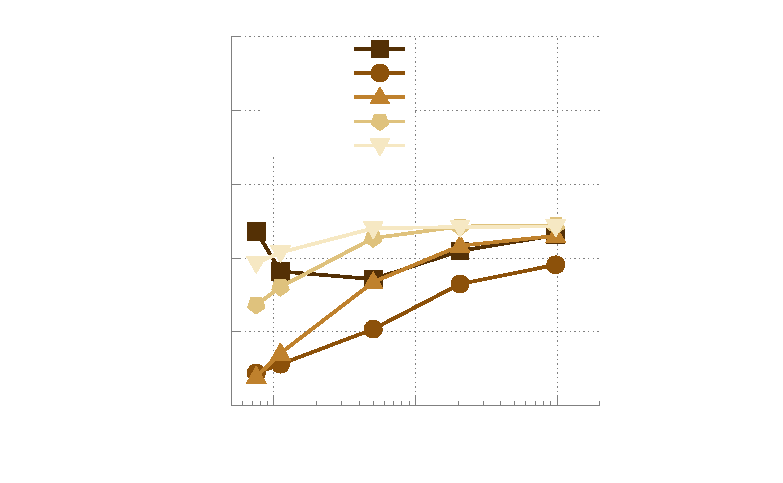
\includegraphics{ratioDragCa}}%
    \gplfronttext
  \end{picture}%
\endgroup

\par\end{centering}
\caption{Ratio of traction ($x$-component) on fluid-fluid interface over traction
on solid-fluid interfaces in UC3 as a function of the capillary number
and for different apertures at steady-state.\label{fig:ratioTractionCa}}
\end{figure}

Consider now the total traction on the fluid-fluid interface and the
total traction exerted upon the solid boundaries plotted separately
against the dimensionless aperture in Fig.~\ref{fig:tractionTotal}.
Between $h^{*}=0.5$ and $h^{*}=0.05$ the traction exerted upon the
solid scale as $h^{-2}$, in contrast the traction at the fluid-fluid
interface increases faster with $h$ over the same interval. This
explains why $T_{f}^{x}/T_{s}^{x}$ increases as the aperture between
the plates decreases. To go further we studied separately the pressure
part and the viscous contribution in Eq.\ref{eq:tractionIntegral}
at the fluid-fluid interface as a function of the dimensionless aperture,
see Fig.~\ref{fig:tractionFluid}. For $h^{*}<0.5$ the pressure
part largely dominates the viscous contribution and the evolution
of the traction is therefore controlled by it. The pressure part scales
as $h^{-2}$ for $Ca=1$ but increases faster when the capillary number
decreases. 

\begin{figure}
\begin{centering}
% GNUPLOT: LaTeX picture with Postscript
\begingroup
  % Encoding inside the plot.  In the header of your document, this encoding
  % should to defined, e.g., by using
  % \usepackage[cp1252,<other encodings>]{inputenc}
  \makeatletter
  \providecommand\color[2][]{%
    \GenericError{(gnuplot) \space\space\space\@spaces}{%
      Package color not loaded in conjunction with
      terminal option `colourtext'%
    }{See the gnuplot documentation for explanation.%
    }{Either use 'blacktext' in gnuplot or load the package
      color.sty in LaTeX.}%
    \renewcommand\color[2][]{}%
  }%
  \providecommand\includegraphics[2][]{%
    \GenericError{(gnuplot) \space\space\space\@spaces}{%
      Package graphicx or graphics not loaded%
    }{See the gnuplot documentation for explanation.%
    }{The gnuplot epslatex terminal needs graphicx.sty or graphics.sty.}%
    \renewcommand\includegraphics[2][]{}%
  }%
  \providecommand\rotatebox[2]{#2}%
  \@ifundefined{ifGPcolor}{%
    \newif\ifGPcolor
    \GPcolortrue
  }{}%
  \@ifundefined{ifGPblacktext}{%
    \newif\ifGPblacktext
    \GPblacktexttrue
  }{}%
  % define a \g@addto@macro without @ in the name:
  \let\gplgaddtomacro\g@addto@macro
  % define empty templates for all commands taking text:
  \gdef\gplbacktext{}%
  \gdef\gplfronttext{}%
  \makeatother
  \ifGPblacktext
    % no textcolor at all
    \def\colorrgb#1{}%
    \def\colorgray#1{}%
  \else
    % gray or color?
    \ifGPcolor
      \def\colorrgb#1{\color[rgb]{#1}}%
      \def\colorgray#1{\color[gray]{#1}}%
      \expandafter\def\csname LTw\endcsname{\color{white}}%
      \expandafter\def\csname LTb\endcsname{\color{black}}%
      \expandafter\def\csname LTa\endcsname{\color{black}}%
      \expandafter\def\csname LT0\endcsname{\color[rgb]{1,0,0}}%
      \expandafter\def\csname LT1\endcsname{\color[rgb]{0,1,0}}%
      \expandafter\def\csname LT2\endcsname{\color[rgb]{0,0,1}}%
      \expandafter\def\csname LT3\endcsname{\color[rgb]{1,0,1}}%
      \expandafter\def\csname LT4\endcsname{\color[rgb]{0,1,1}}%
      \expandafter\def\csname LT5\endcsname{\color[rgb]{1,1,0}}%
      \expandafter\def\csname LT6\endcsname{\color[rgb]{0,0,0}}%
      \expandafter\def\csname LT7\endcsname{\color[rgb]{1,0.3,0}}%
      \expandafter\def\csname LT8\endcsname{\color[rgb]{0.5,0.5,0.5}}%
    \else
      % gray
      \def\colorrgb#1{\color{black}}%
      \def\colorgray#1{\color[gray]{#1}}%
      \expandafter\def\csname LTw\endcsname{\color{white}}%
      \expandafter\def\csname LTb\endcsname{\color{black}}%
      \expandafter\def\csname LTa\endcsname{\color{black}}%
      \expandafter\def\csname LT0\endcsname{\color{black}}%
      \expandafter\def\csname LT1\endcsname{\color{black}}%
      \expandafter\def\csname LT2\endcsname{\color{black}}%
      \expandafter\def\csname LT3\endcsname{\color{black}}%
      \expandafter\def\csname LT4\endcsname{\color{black}}%
      \expandafter\def\csname LT5\endcsname{\color{black}}%
      \expandafter\def\csname LT6\endcsname{\color{black}}%
      \expandafter\def\csname LT7\endcsname{\color{black}}%
      \expandafter\def\csname LT8\endcsname{\color{black}}%
    \fi
  \fi
    \setlength{\unitlength}{0.0500bp}%
    \ifx\gptboxheight\undefined%
      \newlength{\gptboxheight}%
      \newlength{\gptboxwidth}%
      \newsavebox{\gptboxtext}%
    \fi%
    \setlength{\fboxrule}{0.5pt}%
    \setlength{\fboxsep}{1pt}%
\begin{picture}(7180.00,4300.00)%
    \gplgaddtomacro\gplbacktext{%
      \colorrgb{0.50,0.50,0.50}%%
      \put(1625,700){\makebox(0,0)[r]{\strut{}1}}%
      \colorrgb{0.50,0.50,0.50}%%
      \put(1625,1263){\makebox(0,0)[r]{\strut{}\(1.0 \times 10^{1}\)}}%
      \colorrgb{0.50,0.50,0.50}%%
      \put(1625,1827){\makebox(0,0)[r]{\strut{}\(1.0 \times 10^{2}\)}}%
      \colorrgb{0.50,0.50,0.50}%%
      \put(1625,2390){\makebox(0,0)[r]{\strut{}\(1.0 \times 10^{3}\)}}%
      \colorrgb{0.50,0.50,0.50}%%
      \put(1625,2953){\makebox(0,0)[r]{\strut{}\(1.0 \times 10^{4}\)}}%
      \colorrgb{0.50,0.50,0.50}%%
      \put(1625,3517){\makebox(0,0)[r]{\strut{}\(1.0 \times 10^{5}\)}}%
      \colorrgb{0.50,0.50,0.50}%%
      \put(1625,4080){\makebox(0,0)[r]{\strut{}\(1.0 \times 10^{6}\)}}%
      \colorrgb{0.50,0.50,0.50}%%
      \put(2793,481){\makebox(0,0){\strut{}$0.1$}}%
      \colorrgb{0.50,0.50,0.50}%%
      \put(4840,481){\makebox(0,0){\strut{}$1$}}%
      \colorrgb{0.50,0.50,0.50}%%
      \put(6888,481){\makebox(0,0){\strut{}$10$}}%
      \csname LTb\endcsname%%
      \put(1978,4025){\makebox(0,0)[l]{\strut{}$2^{\mathrm{nd}}\:\mathrm{order}$}}%
    }%
    \gplgaddtomacro\gplfronttext{%
      \csname LTb\endcsname%%
      \put(473,2390){\rotatebox{-270}{\makebox(0,0){\strut{}$T_{i}^x\:(\mathrm{N/m^3})$}}}%
      \csname LTb\endcsname%%
      \put(4305,153){\makebox(0,0){\strut{}$h^*$}}%
      \csname LTb\endcsname%%
      \put(6122,3856){\makebox(0,0)[r]{\strut{}$Ca=1 \times 10^{0},s$}}%
      \csname LTb\endcsname%%
      \put(6122,3583){\makebox(0,0)[r]{\strut{}$-,f$}}%
      \csname LTb\endcsname%%
      \put(6122,3310){\makebox(0,0)[r]{\strut{}$Ca=5 \times 10^{-2},s$}}%
      \csname LTb\endcsname%%
      \put(6122,3037){\makebox(0,0)[r]{\strut{}$-,f$}}%
      \csname LTb\endcsname%%
      \put(6122,2764){\makebox(0,0)[r]{\strut{}$Ca=7.5 \times 10^{-3},s$}}%
      \csname LTb\endcsname%%
      \put(6122,2491){\makebox(0,0)[r]{\strut{}$-,f$}}%
    }%
    \gplbacktext
    \put(0,0){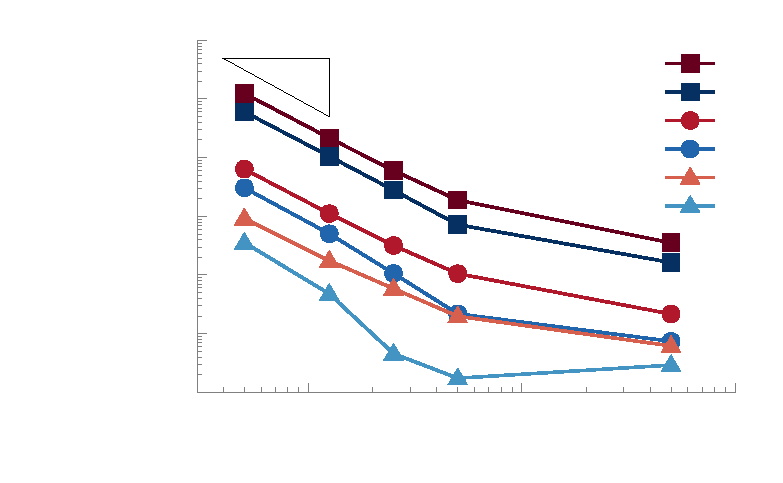
\includegraphics{tractionTotal}}%
    \gplfronttext
  \end{picture}%
\endgroup

\par\end{centering}
\caption{$x$-component of the traction exerted upon fluid-fluid interface
and upon the solid-fluid interface in UC3 as a function of the dimensionless
aperture between the Hele-Shaw plates and for different capillary
numbers at steady-state.\label{fig:tractionTotal}}
\end{figure}

\begin{figure}
\begin{centering}
% GNUPLOT: LaTeX picture with Postscript
\begingroup
  % Encoding inside the plot.  In the header of your document, this encoding
  % should to defined, e.g., by using
  % \usepackage[cp1252,<other encodings>]{inputenc}
  \makeatletter
  \providecommand\color[2][]{%
    \GenericError{(gnuplot) \space\space\space\@spaces}{%
      Package color not loaded in conjunction with
      terminal option `colourtext'%
    }{See the gnuplot documentation for explanation.%
    }{Either use 'blacktext' in gnuplot or load the package
      color.sty in LaTeX.}%
    \renewcommand\color[2][]{}%
  }%
  \providecommand\includegraphics[2][]{%
    \GenericError{(gnuplot) \space\space\space\@spaces}{%
      Package graphicx or graphics not loaded%
    }{See the gnuplot documentation for explanation.%
    }{The gnuplot epslatex terminal needs graphicx.sty or graphics.sty.}%
    \renewcommand\includegraphics[2][]{}%
  }%
  \providecommand\rotatebox[2]{#2}%
  \@ifundefined{ifGPcolor}{%
    \newif\ifGPcolor
    \GPcolortrue
  }{}%
  \@ifundefined{ifGPblacktext}{%
    \newif\ifGPblacktext
    \GPblacktexttrue
  }{}%
  % define a \g@addto@macro without @ in the name:
  \let\gplgaddtomacro\g@addto@macro
  % define empty templates for all commands taking text:
  \gdef\gplbacktext{}%
  \gdef\gplfronttext{}%
  \makeatother
  \ifGPblacktext
    % no textcolor at all
    \def\colorrgb#1{}%
    \def\colorgray#1{}%
  \else
    % gray or color?
    \ifGPcolor
      \def\colorrgb#1{\color[rgb]{#1}}%
      \def\colorgray#1{\color[gray]{#1}}%
      \expandafter\def\csname LTw\endcsname{\color{white}}%
      \expandafter\def\csname LTb\endcsname{\color{black}}%
      \expandafter\def\csname LTa\endcsname{\color{black}}%
      \expandafter\def\csname LT0\endcsname{\color[rgb]{1,0,0}}%
      \expandafter\def\csname LT1\endcsname{\color[rgb]{0,1,0}}%
      \expandafter\def\csname LT2\endcsname{\color[rgb]{0,0,1}}%
      \expandafter\def\csname LT3\endcsname{\color[rgb]{1,0,1}}%
      \expandafter\def\csname LT4\endcsname{\color[rgb]{0,1,1}}%
      \expandafter\def\csname LT5\endcsname{\color[rgb]{1,1,0}}%
      \expandafter\def\csname LT6\endcsname{\color[rgb]{0,0,0}}%
      \expandafter\def\csname LT7\endcsname{\color[rgb]{1,0.3,0}}%
      \expandafter\def\csname LT8\endcsname{\color[rgb]{0.5,0.5,0.5}}%
    \else
      % gray
      \def\colorrgb#1{\color{black}}%
      \def\colorgray#1{\color[gray]{#1}}%
      \expandafter\def\csname LTw\endcsname{\color{white}}%
      \expandafter\def\csname LTb\endcsname{\color{black}}%
      \expandafter\def\csname LTa\endcsname{\color{black}}%
      \expandafter\def\csname LT0\endcsname{\color{black}}%
      \expandafter\def\csname LT1\endcsname{\color{black}}%
      \expandafter\def\csname LT2\endcsname{\color{black}}%
      \expandafter\def\csname LT3\endcsname{\color{black}}%
      \expandafter\def\csname LT4\endcsname{\color{black}}%
      \expandafter\def\csname LT5\endcsname{\color{black}}%
      \expandafter\def\csname LT6\endcsname{\color{black}}%
      \expandafter\def\csname LT7\endcsname{\color{black}}%
      \expandafter\def\csname LT8\endcsname{\color{black}}%
    \fi
  \fi
    \setlength{\unitlength}{0.0500bp}%
    \ifx\gptboxheight\undefined%
      \newlength{\gptboxheight}%
      \newlength{\gptboxwidth}%
      \newsavebox{\gptboxtext}%
    \fi%
    \setlength{\fboxrule}{0.5pt}%
    \setlength{\fboxsep}{1pt}%
\begin{picture}(7900.00,7900.00)%
    \gplgaddtomacro\gplbacktext{%
      \colorrgb{0.50,0.50,0.50}%%
      \put(1625,4650){\makebox(0,0)[r]{\strut{}\(1.0 \times 10^{1}\)}}%
      \colorrgb{0.50,0.50,0.50}%%
      \put(1625,5408){\makebox(0,0)[r]{\strut{}\(1.0 \times 10^{2}\)}}%
      \colorrgb{0.50,0.50,0.50}%%
      \put(1625,6165){\makebox(0,0)[r]{\strut{}\(1.0 \times 10^{3}\)}}%
      \colorrgb{0.50,0.50,0.50}%%
      \put(1625,6923){\makebox(0,0)[r]{\strut{}\(1.0 \times 10^{4}\)}}%
      \colorrgb{0.50,0.50,0.50}%%
      \put(1625,7680){\makebox(0,0)[r]{\strut{}\(1.0 \times 10^{5}\)}}%
      \colorrgb{0.50,0.50,0.50}%%
      \put(2013,4431){\makebox(0,0){\strut{}$0.1$}}%
      \colorrgb{0.50,0.50,0.50}%%
      \put(2981,4431){\makebox(0,0){\strut{}$1$}}%
      \csname LTb\endcsname%%
      \put(2690,6888){\makebox(0,0)[l]{\strut{}$Ca=1$}}%
      \csname LTb\endcsname%%
      \put(2013,5997){\makebox(0,0)[l]{\strut{}$2$}}%
    }%
    \gplgaddtomacro\gplfronttext{%
      \csname LTb\endcsname%%
      \put(473,6165){\rotatebox{-270}{\makebox(0,0){\strut{}$T_{f}^x\:(\mathrm{N/m^3})$}}}%
      \csname LTb\endcsname%%
      \put(2690,4103){\makebox(0,0){\strut{}$h^*$}}%
      \csname LTb\endcsname%%
      \put(2892,7483){\makebox(0,0)[r]{\strut{}$viscous$}}%
      \csname LTb\endcsname%%
      \put(2892,7264){\makebox(0,0)[r]{\strut{}$pressure$}}%
    }%
    \gplgaddtomacro\gplbacktext{%
      \colorrgb{0.50,0.50,0.50}%%
      \put(5356,4388){\makebox(0,0)[r]{\strut{}1}}%
      \colorrgb{0.50,0.50,0.50}%%
      \put(5356,5211){\makebox(0,0)[r]{\strut{}\(1.0 \times 10^{1}\)}}%
      \colorrgb{0.50,0.50,0.50}%%
      \put(5356,6034){\makebox(0,0)[r]{\strut{}\(1.0 \times 10^{2}\)}}%
      \colorrgb{0.50,0.50,0.50}%%
      \put(5356,6857){\makebox(0,0)[r]{\strut{}\(1.0 \times 10^{3}\)}}%
      \colorrgb{0.50,0.50,0.50}%%
      \put(5356,7680){\makebox(0,0)[r]{\strut{}\(1.0 \times 10^{4}\)}}%
      \colorrgb{0.50,0.50,0.50}%%
      \put(5777,4169){\makebox(0,0){\strut{}$0.1$}}%
      \colorrgb{0.50,0.50,0.50}%%
      \put(6855,4169){\makebox(0,0){\strut{}$1$}}%
      \csname LTb\endcsname%%
      \put(6531,6819){\makebox(0,0)[l]{\strut{}$Ca=0.05$}}%
    }%
    \gplgaddtomacro\gplfronttext{%
      \csname LTb\endcsname%%
      \put(6842,7483){\makebox(0,0)[r]{\strut{}$viscous$}}%
      \csname LTb\endcsname%%
      \put(6842,7264){\makebox(0,0)[r]{\strut{}$pressure$}}%
    }%
    \gplgaddtomacro\gplbacktext{%
      \colorrgb{0.50,0.50,0.50}%%
      \put(1503,1755){\makebox(0,0)[r]{\strut{}1}}%
      \colorrgb{0.50,0.50,0.50}%%
      \put(1503,438){\makebox(0,0)[r]{\strut{}\(1.0 \times 10^{-2}\)}}%
      \colorrgb{0.50,0.50,0.50}%%
      \put(1503,1097){\makebox(0,0)[r]{\strut{}\(1.0 \times 10^{-1}\)}}%
      \colorrgb{0.50,0.50,0.50}%%
      \put(1503,2414){\makebox(0,0)[r]{\strut{}\(1.0 \times 10^{1}\)}}%
      \colorrgb{0.50,0.50,0.50}%%
      \put(1503,3072){\makebox(0,0)[r]{\strut{}\(1.0 \times 10^{2}\)}}%
      \colorrgb{0.50,0.50,0.50}%%
      \put(1503,3731){\makebox(0,0)[r]{\strut{}\(1.0 \times 10^{3}\)}}%
      \colorrgb{0.50,0.50,0.50}%%
      \put(1910,219){\makebox(0,0){\strut{}$0.1$}}%
      \colorrgb{0.50,0.50,0.50}%%
      \put(2939,219){\makebox(0,0){\strut{}$1$}}%
      \csname LTb\endcsname%%
      \put(2629,2970){\makebox(0,0)[l]{\strut{}$Ca=0.01$}}%
    }%
    \gplgaddtomacro\gplfronttext{%
      \csname LTb\endcsname%%
      \put(2892,3534){\makebox(0,0)[r]{\strut{}$viscous$}}%
      \csname LTb\endcsname%%
      \put(2892,3315){\makebox(0,0)[r]{\strut{}$pressure$}}%
    }%
    \gplgaddtomacro\gplbacktext{%
      \colorrgb{0.50,0.50,0.50}%%
      \put(5453,1261){\makebox(0,0)[r]{\strut{}1}}%
      \colorrgb{0.50,0.50,0.50}%%
      \put(5453,438){\makebox(0,0)[r]{\strut{}\(1.0 \times 10^{-1}\)}}%
      \colorrgb{0.50,0.50,0.50}%%
      \put(5453,2085){\makebox(0,0)[r]{\strut{}\(1.0 \times 10^{1}\)}}%
      \colorrgb{0.50,0.50,0.50}%%
      \put(5453,2908){\makebox(0,0)[r]{\strut{}\(1.0 \times 10^{2}\)}}%
      \colorrgb{0.50,0.50,0.50}%%
      \put(5453,3731){\makebox(0,0)[r]{\strut{}\(1.0 \times 10^{3}\)}}%
      \colorrgb{0.50,0.50,0.50}%%
      \put(5860,219){\makebox(0,0){\strut{}$0.1$}}%
      \colorrgb{0.50,0.50,0.50}%%
      \put(6889,219){\makebox(0,0){\strut{}$1$}}%
      \csname LTb\endcsname%%
      \put(6351,2870){\makebox(0,0)[l]{\strut{}$Ca=0.0075$}}%
      \csname LTb\endcsname%%
      \put(6729,2085){\makebox(0,0)[l]{\strut{}$2$}}%
    }%
    \gplgaddtomacro\gplfronttext{%
      \csname LTb\endcsname%%
      \put(6842,3534){\makebox(0,0)[r]{\strut{}$viscous$}}%
      \csname LTb\endcsname%%
      \put(6842,3315){\makebox(0,0)[r]{\strut{}$pressure$}}%
    }%
    \gplbacktext
    \put(0,0){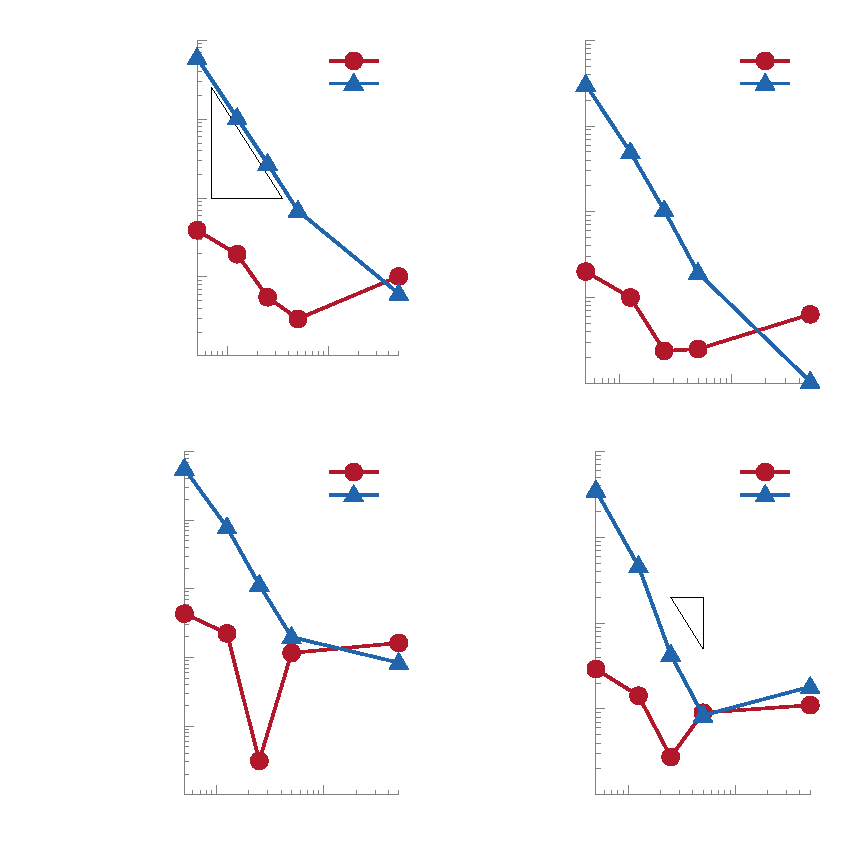
\includegraphics{multiplotTractionFluidInterface}}%
    \gplfronttext
  \end{picture}%
\endgroup

\par\end{centering}
\caption{Viscous and pressure part of $x$-component of the traction exerted
upon the fluid-fluid interface in UC3 as a function of the dimensionless
aperture between the Hele-Shaw plates at steady-state for different
capillary numbers.\label{fig:tractionFluid}}
\end{figure}

Due to the proximity of the plates, the frictional forces are high,
and they become higher and higher as they get closer. However, the
traction exerted at the fluid/fluid interface does not become negligible
compared to that exerted by the fluid upon the solid. Clearly, what
is happening here is that the pressure increases due to the combination
of constant inlet velocity and lower absolute permeability have a
stronger effect on the traction term exerted at the fluid-fluid boundary. -

\newpage{}

\bibliographystyle{elsarticle-harv}
\bibliography{biblio}

\newpage{}


\appendix

\section{Model validation}

The code is validated by comparison with a Boundary-Element Method,
which relies on a surface discretization of the interface and a pseudo-analytical
formulation in the bulk of the phases. This allows us to precisely
locate the interface, even in the case of very thin film flow, and
to carefully analyze the choice of parameters in Eq.~\ref{eq:advecPhi}.
\end{document}
